%!TEX root = ../template.tex
%%%%%%%%%%%%%%%%%%%%%%%%%%%%%%%%%%%%%%%%%%%%%%%%%%%%%%%%%%%%%%%%%%%
%% chapter1.tex
%% NOVA thesis document file
%%
%% Chapter with introduciton


\chapter{Design and Implementation}
\label{cha:design_and_implementation}

The design process adopted was an iterative design approach to build iteratively the solution according to the users' acceptance and feedback retrieved during users test in each iteration. Throughout this chapter, it is detailed all design and implementation decisions considered in order to reach the final prototype.

\section{Sketching}
\label{sec:sketching}

Before starting the development of the interface prototypes which were tested with users, some sketches were performed in order to organize and explore ideas to tackle the existing usability problems. The most important to reach in the final of this phase was not a functional or complete interface, but some practical ideas that could be applied in the following prototypes.

Considering the extensive list of problems identified, prioritization was an important aspect taken into account throughout all design phases. The first problem explored was the difficulty to comprehend what is the database query purpose.

In the existing interface, users do not have a unique and clear view that facilitates the comprehension of what data could be fetched from the database through the query presented. As illustrated in Figure \ref{fig:example_of_query_representation}, the user can only see some components of the query at a time, due to the usage of tabs to individualize each type of query components. In addition, as can be observed in Figure \ref{fig:ss_existing_layout}, when users open the query, only the query output preview was shown. That was considered a problem in the analysis of the interface for two different points of view:

\begin{itemize}
    \item When the existing interface was tested with users who do not usually use the Platform, they did not easily find out the existence of the tabs and tried to perceive the query purpose only observing the data preview. Besides not being an effective understanding technique, it can be even more difficult when the output contains several columns;
    \item The users accustomed to this data tool revealed that is cumbersome to open and navigate between tabs in order to understand the query.
\end{itemize}

\begin{figure}[tb]
    \centering
    \subcaptionbox{Starting point (only the result is visible)\label{fig:ss_existing_layout}}%
      {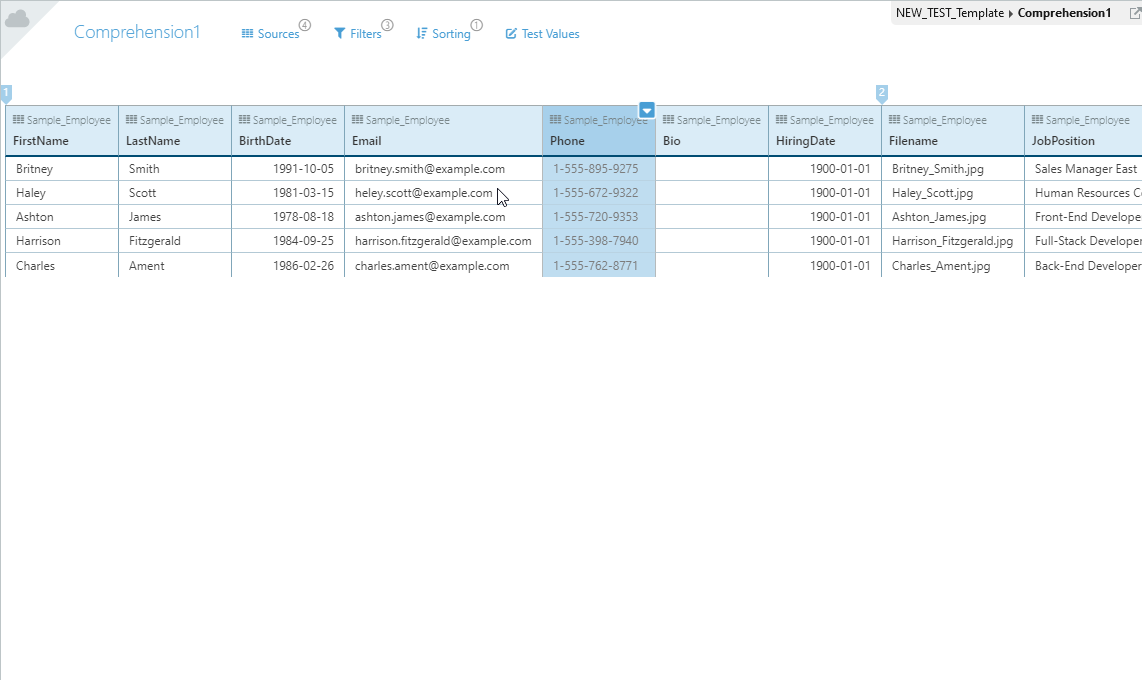
\includegraphics[width=0.5\linewidth]{ss-existing-layout}}%
    \subcaptionbox{Sources Tab\label{fig:ss_existing_layout_sources}}%
      {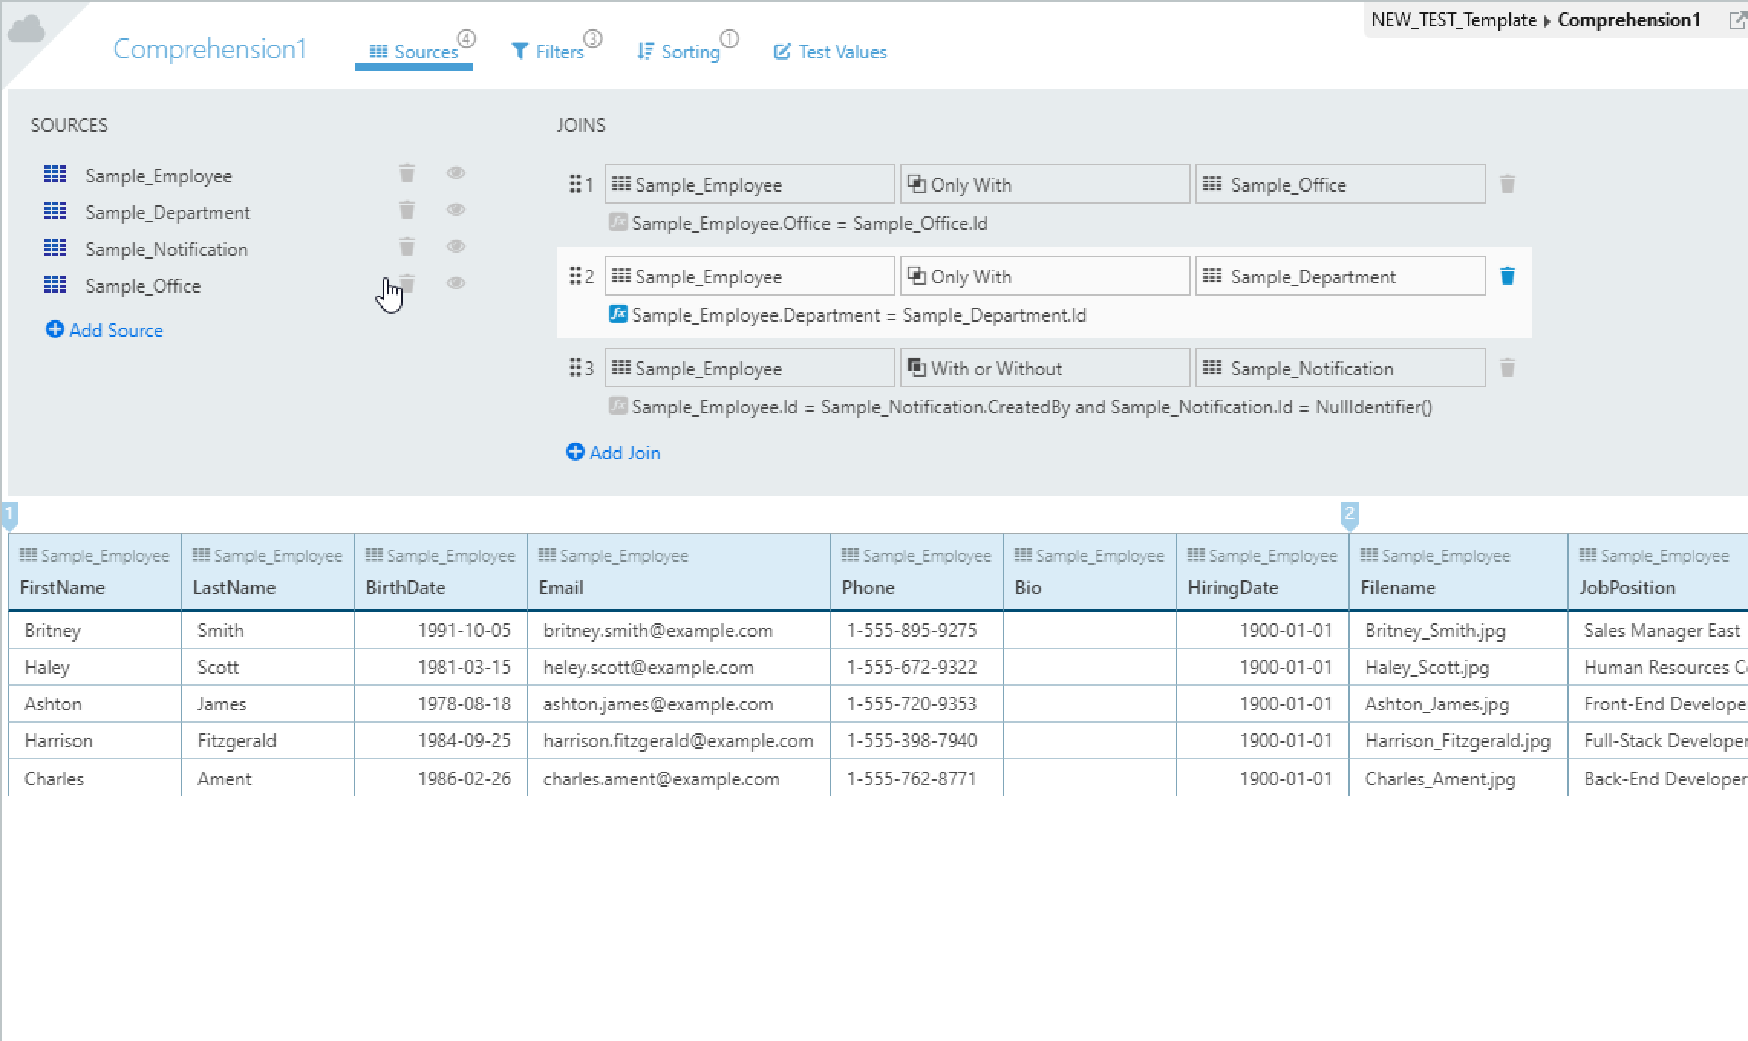
\includegraphics[width=0.5\linewidth]{ss-existing-layout-sources}}%
      \\
    \subcaptionbox{Filters Tab\label{fig:ss_existing_layout_filters}}%
    {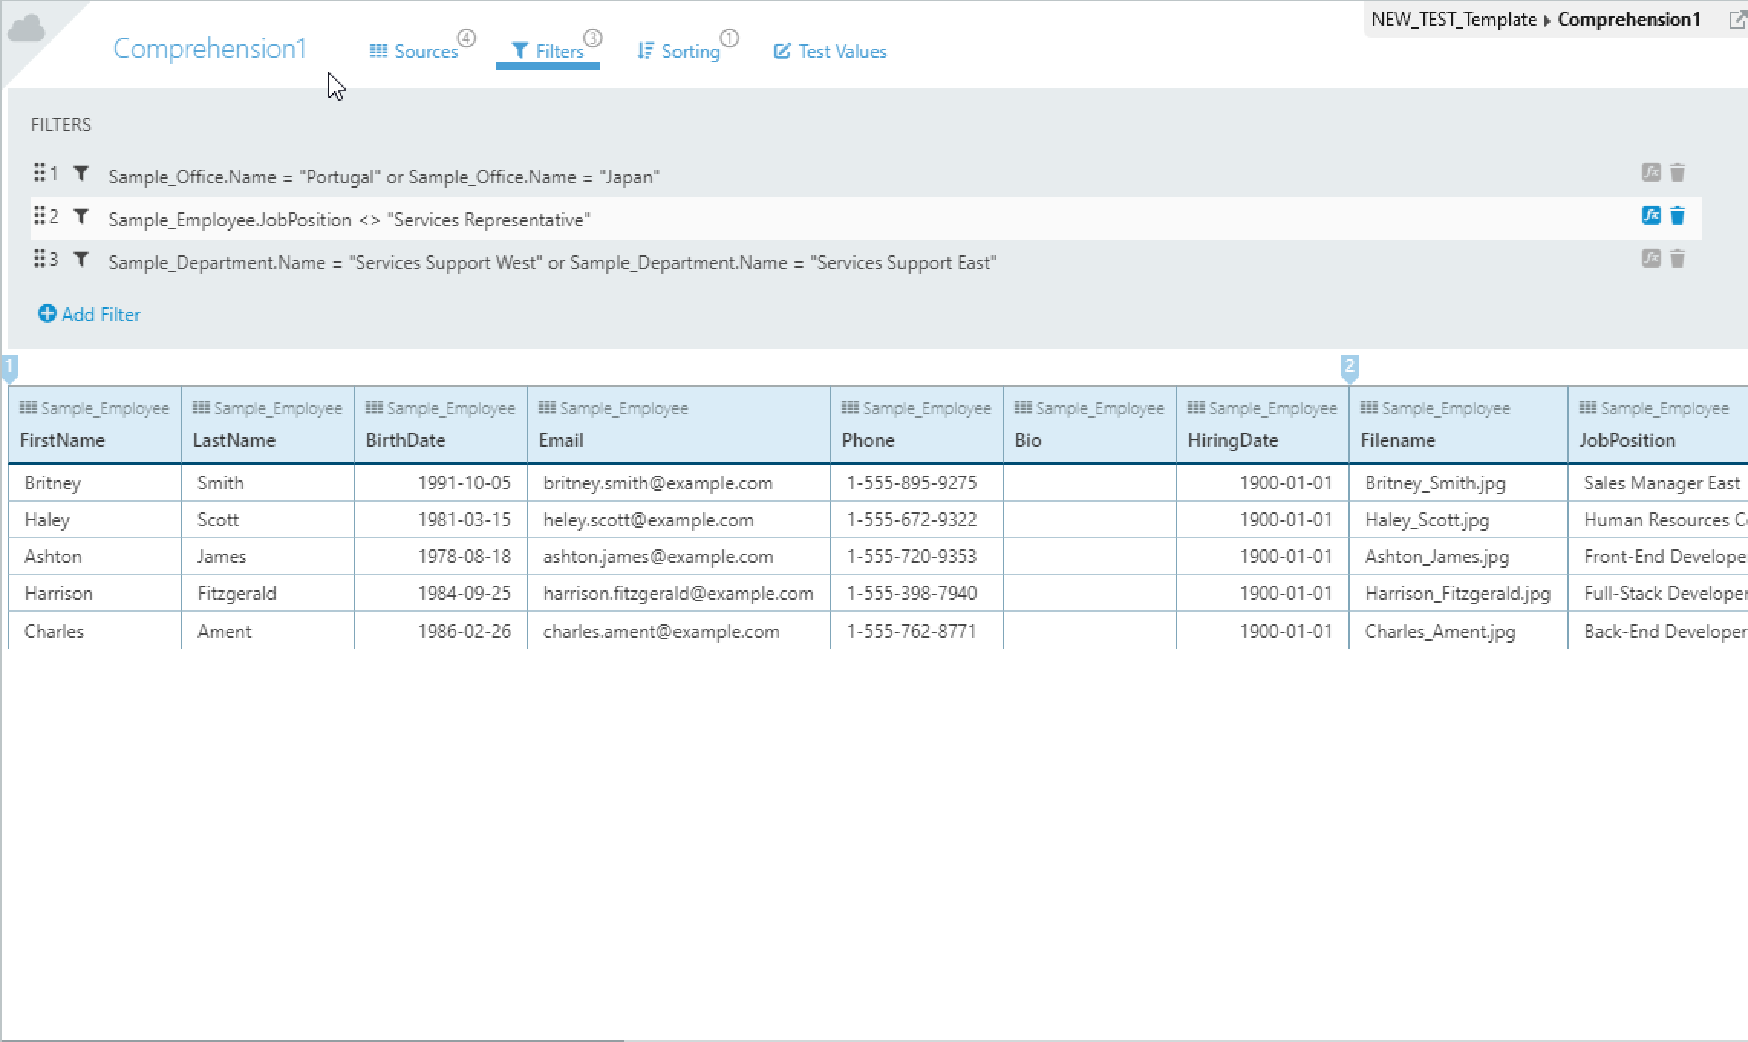
\includegraphics[width=0.5\linewidth]{ss-existing-layout-filters}}%
  \subcaptionbox{Sorting Tab\label{fig:ss_existing_layout_sorting}}%
    {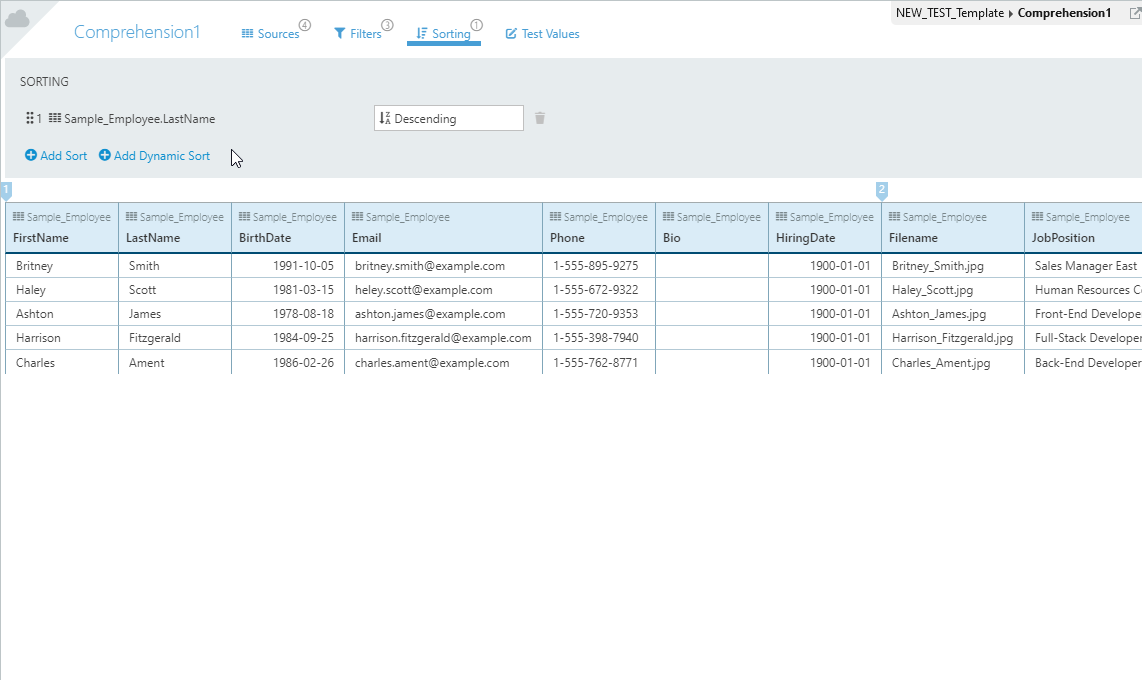
\includegraphics[width=0.5\linewidth]{ss-existing-layout-sorting}}%
  \caption{Example of a database query representation through the existing visual interface.}
    \label{fig:example_of_query_representation}
\end{figure}

Therefore, the designing of a new general layout where it is possible to view the most important query components at once was considered a major requirement. A solid improvement regarding that, could optimize not only the time and effort required to comprehend queries but also to formulate them, since all information is more visible and accessible.

There was also a concern to build a layout that does not compromise the system usability for more complex cases, such as queries that contain a relevant number of entities or conditions.

Accordingly, some wireframes were sketched in order to percept how the query components could be jointly combined in a unique view. Figure \ref{fig:sketch_wireframes} illustrates the two options elected from multiple approaches explored.

In both options, there are two principal areas in the interface as it was before: the query editor area and the preview of the query result. However, it was explored two new manners to display all information of editors jointly with the query result preview. In \nameref{fig:sketch_wireframe_a}, the sub-editors remain in the top area and the query result preview below. The \nameref{fig:sketch_wireframe_b} illustrates another possibility sketched where all editors are presented on the left side of the screen and the visualization of the results are presented on the right side.

\begin{figure}[tb]
  \centering
  \subcaptionbox{Option A\label{fig:sketch_wireframe_a}}%
    {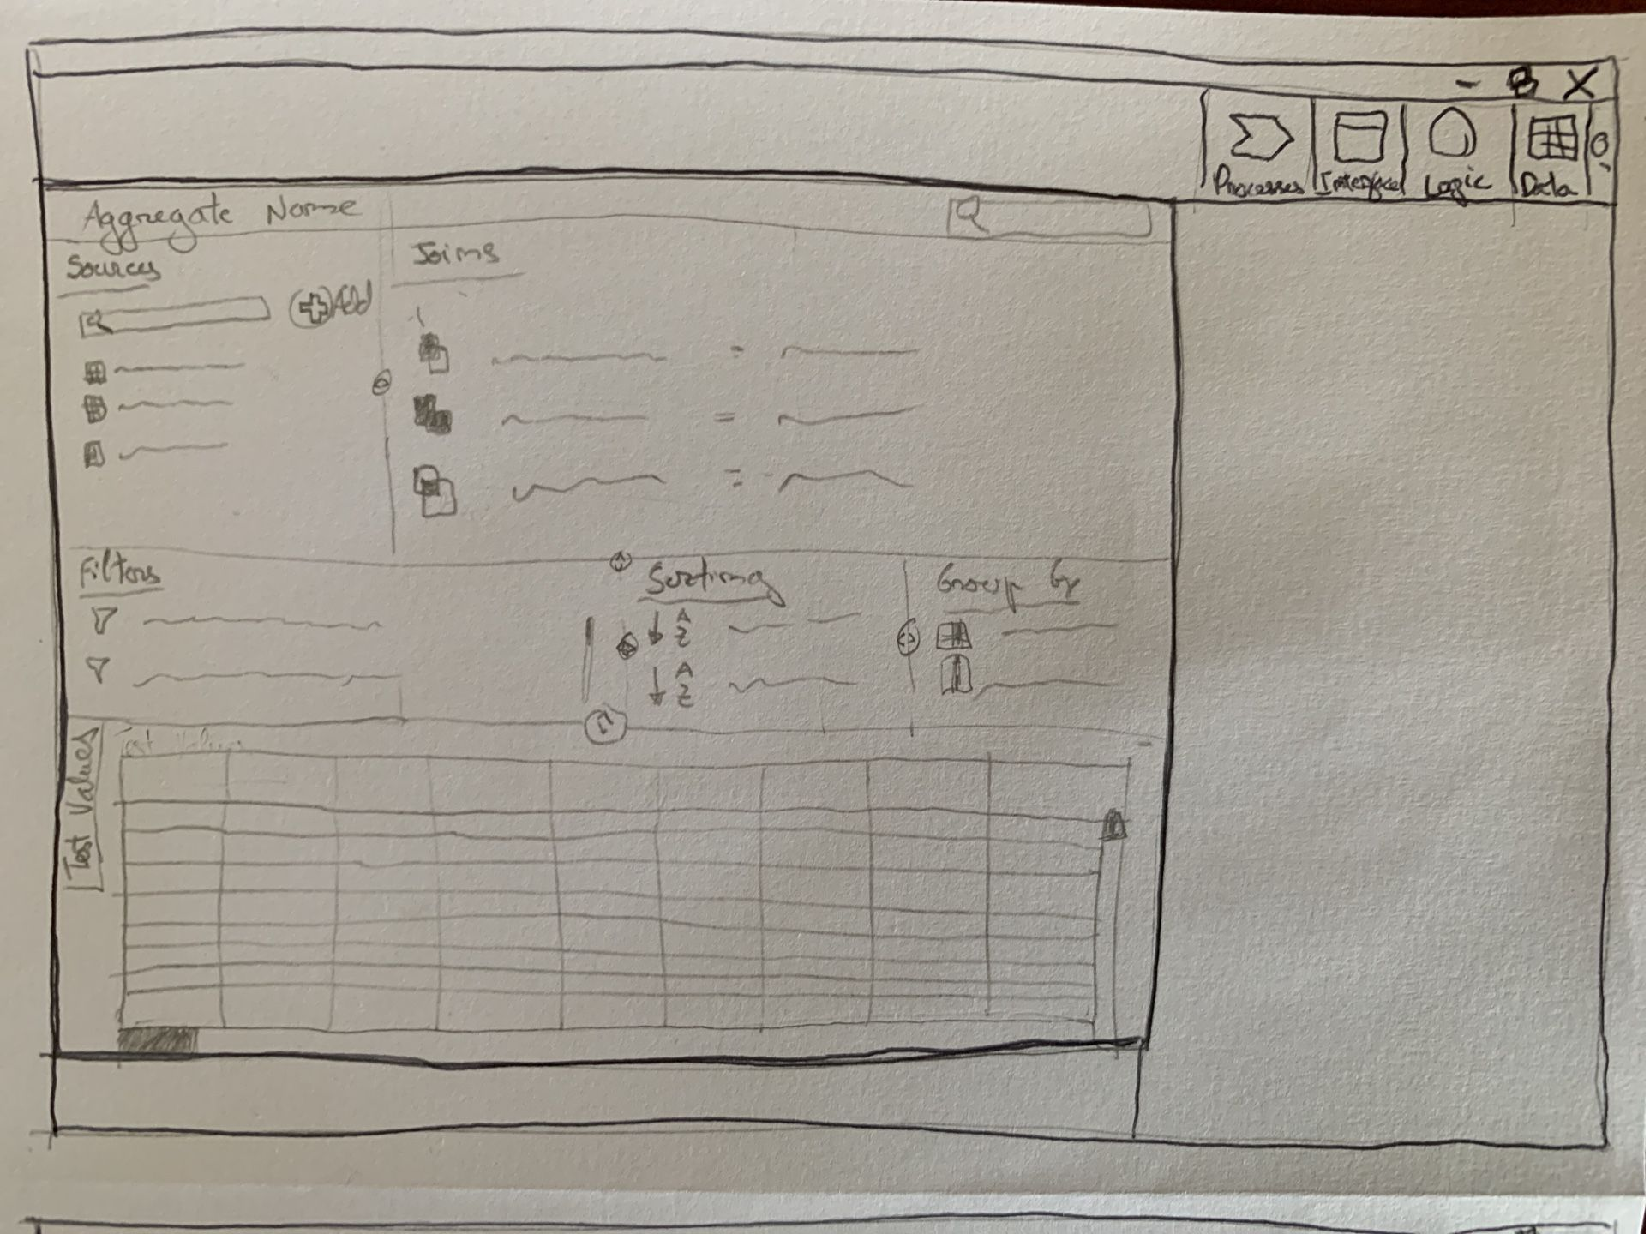
\includegraphics[width=0.5\linewidth]{sketch-wireframe-a}}%
  \subcaptionbox{Option B\label{fig:sketch_wireframe_b}}%
  {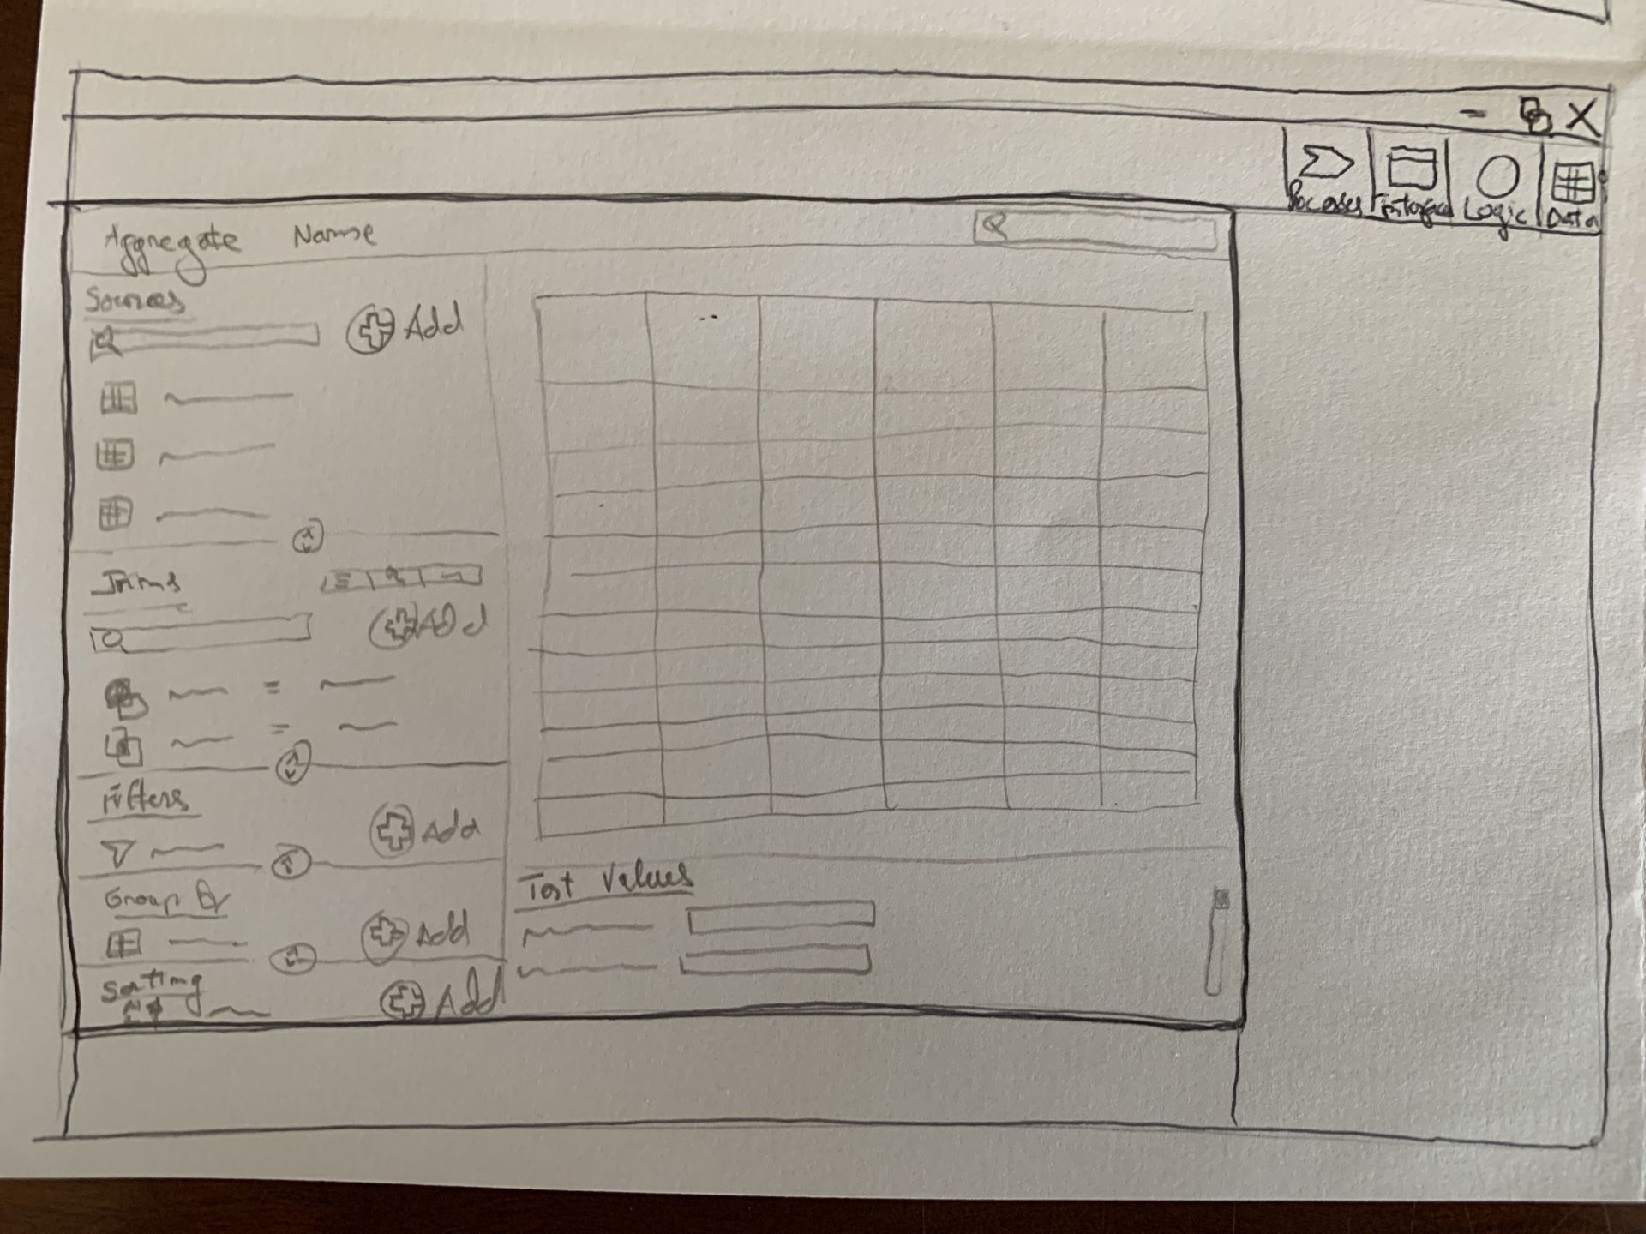
\includegraphics[width=0.5\linewidth]{sketch-wireframe-b}}%
\caption{Interface layout sketches.}
  \label{fig:sketch_wireframes}
\end{figure}

Regardless of the option, the layouts presented have in a single view the most important aspects to understand what query is built.

Beyond the disposition of the different interface views and components, other features were sketched in order to think more about it and structure concrete ideas to implement it.

The existing interface has no mechanism that allows the user to easily find the data of an entity or attribute. The attributes included in the query were not represented in any region of the interface beyond the query result table. Thereby, the unique way to find out the attribute is looking for in each table header, using the horizontal scroll, until the intended attribute is found. That process is cumbersome and slow, so that an alternative which includes the attributes in the sources view was sketched. Consequently, users can click on an attribute and the attribute will be highlighted automatically in the query result preview, as illustrated in Figure \ref{fig:sketchAttributeSearch}. Also, the idea of a search engine was considered, so that users can search for an entity or attribute faster.

\begin{figure}[htbp]
	\centering
	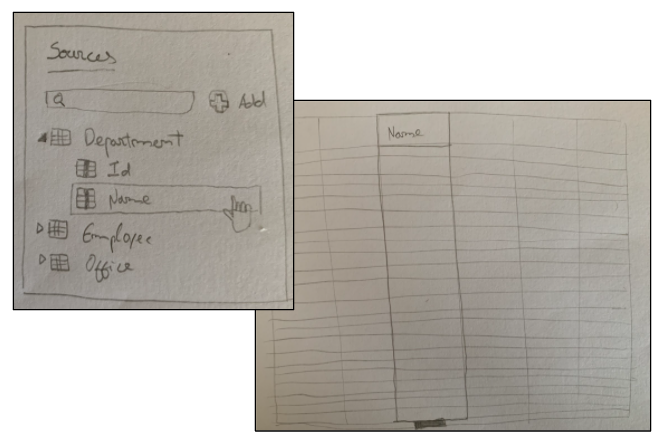
\includegraphics[height=2.5in]{sketch-attribute-search}
	\caption{Searching for an attribute data on the query output preview.}
	\label{fig:sketchAttributeSearch}
\end{figure}

Furthermore, different approaches more compact and functional were explored to display the joins used in the query. Figure \ref{fig:sketchJoins} shows the idea sketched to represent joins in three different lists: a simple list of all join operations inside the query, and two other ones aggregated by the entities involved by the join kind.

\begin{figure}[tb]
  \centering
  \subcaptionbox{Joins flat list\label{fig:sketch-joins-list}}%
    {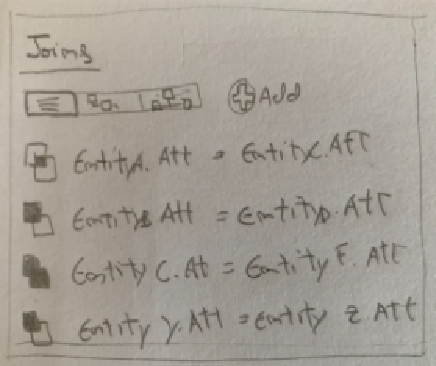
\includegraphics[width=0.3\linewidth]{sketch-joins-list}}%
  \subcaptionbox{Joins associated to each entity\label{fig:sketch-joins-by-entity}}%
  {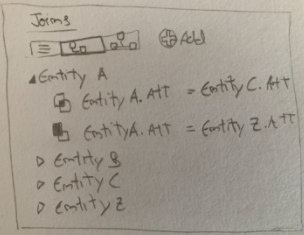
\includegraphics[width=0.3\linewidth]{sketch-joins-by-entity}}%
  \subcaptionbox{Joins by each join kind\label{fig:sketch-joins-by-kind}}%
  {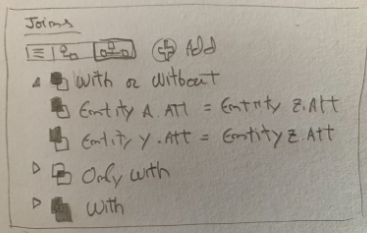
\includegraphics[width=0.3\linewidth]{sketch-joins-by-kind}}%
\caption{Sketches elaborated to explore other approaches to represent the join operations present in the query.}
  \label{fig:sketchJoins}
\end{figure}

Lastly, an idea to accelerate the searching process of a specific element inside the query was sketched. Therefore, the sketch represented in Figure \ref{fig:sketchGeneralSearch} demonstrates an idea taken into account to find all references of an entity. This general search could allow users to find entities, joins, filters, or other query elements faster.

\begin{figure}[htbp]
	\centering
	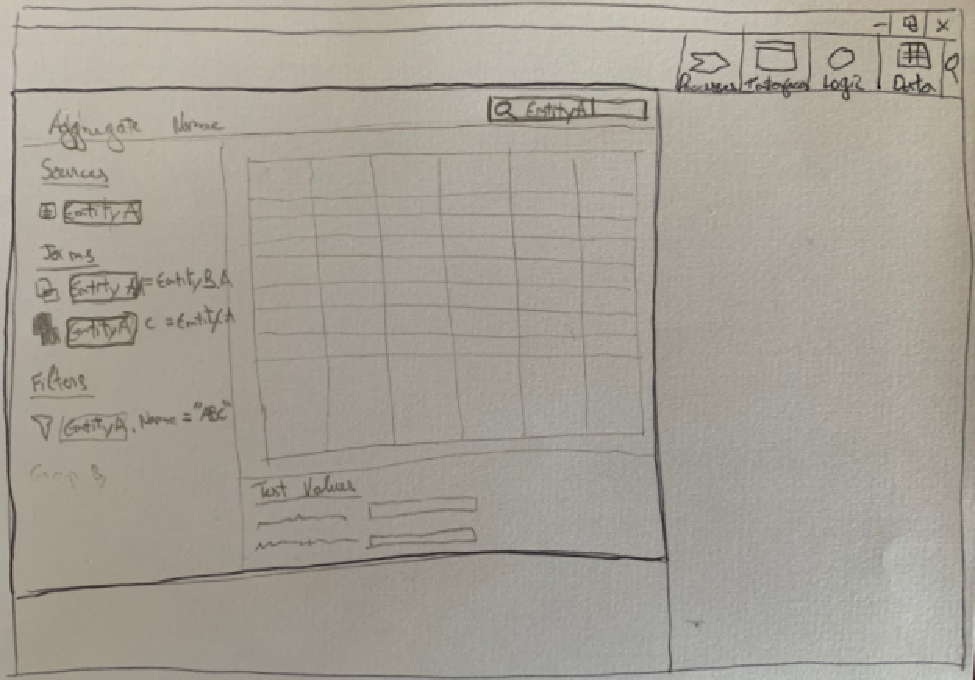
\includegraphics[height=2.5in]{sketch-general-search}
	\caption{Sketch of a general search to allow users to find query elements represented in the interface.}
	\label{fig:sketchGeneralSearch}
\end{figure}

Although the sketched ideas may not be applied to the final prototype since they depend on the whole iterative design process that started afterward, they were important to move the focus from problem definition to solution design.


\section{Paper Prototype}
\label{sec:paper_prototype}
The interactive design process of the solution started in its entirety with the first prototype developed: the paper prototype. The main goal of this phase is the building of a functional prototype implemented in paper using a ruler, a set square, and writing materials, in order to create faster and with a low-risk level a prototype that could be testes by users.

However, due to the COVID-19 pandemic, the prototype was adapted since it was not possible to test the prototype in person. Accordingly, the prototype was scanned and the interactions were configured using the digital product design platform InVision \cite{invision}.
% Do not forget to refer that due to COVID-19 the Paper Prototype was scanned and mounted as a low-fidelity prototype using InVision App.

\subsection{Design}
\label{subsec:paper_prototype_design}
The building process of this low-fidelity prototype started with a design phase where brainstorming took place in order to establish the design priorities for the paper prototype as well as concrete ideas to apply the solutions thought.

\medskip

\textbf{Sub-editors arrangement:}

\medskip

Taking into account the sketches mentioned in the last section, the first question evaluated was which rearrangement of the sub-editors and the result preview views would be implemented in the next phase. In order to take action in this regard, there was a point in the visual query builder background considered. As mentioned in \ref{subsubsec:previous_work}, this querying interface was completely redesigned seven years ago, which had a negative repercussion on users since they were accustomed to the previous interface. Therefore, there was a concern to change the interface without removing the main points that characterize and identify it. In such a way that users would not feel using a completely new interface but an improved version of the existing one.

Comparing the two sketched options (Figure \ref{fig:sketch_wireframes}) with the existing interface (Figure \ref{fig:example_of_query_representation}), the \nameref{fig:sketch_wireframe_a} is the most similar because the editors area keeps on the top region of the interface and the query result data below. For this reason, this arrangement would be considered in the next phase.

Having chosen where would take place the edition area of the interface, the second aspect taken into consideration was how to organize its sub-editors. This decision was taken bearing in mind what each query aspect represents in the user's mental model when they formulate queries as well as the physical space of the interface they could occupy.

In this regard, it was thought about what are the order of the query elements that arise in user thinking. This reasoning was performed taking into consideration the formulation using \gls{SQL} since one of the main goals is the improvement of the interface experience for users that are proficient in \gls{SQL}. According to the conceptual models presented in \ref{sec:query_conceptual_models}, the first aspect the user thinks, after understanding what data is required, is how to translate them to the query language. In \gls{SQL}, the core statements are presented in the following order:

\begin{enumerate}
  \item \textbf{SELECT: }Indicates which attributes will be selected to be present in the query output table;
  \item \textbf{FROM: }Sets out which entities are used to query data. Thereby, even it is necessary to merge tables, the join operations are specified through that statement;
  \item \textbf{WHERE: }Contains the boolean conditions that would filter the results.
  \item \textbf{ORDER BY: }Specify the criteria to order the data gathered.
\end{enumerate}

In this visual query building tool users do not select attributes because there is an optimizing background task that will inspect where the query is used and only select the attributes that will be used. Therefore, in this system, the information specified through the SELECT statement will not be specified by the user.

However, the three other aspects of the query are clearly specified by users in three different interface areas: Sources, Filters, and Sorting respectively. Accordingly, the arrangement chosen to display these three sub-editors follows this logic. The query edition area were divided into two columns. The left side was elected to represent the sources of the query and the right side lists the filters and sorting criteria.

\medskip

\textbf{New approach to represent sources and joins:}

\medskip

Nevertheless, the way entities and joins were presented in the interface, in the previous sources tab, required to be redesigned from scratch. As can be observed in Figure \ref{fig:ss_existing_layout_sources}, a simple list of the entities used was presented in the left side of the editor area and the joins used to merge them in its right side.

Even though some designs regarding that were elaborated in the sketching phase (Figure \ref{fig:sketchJoins}), it was concluded that the main issues remain:

\begin{itemize}
  \item Difficulty to comprehend faster and with a low-effort what entities were integrated into the query. Being a visual interface, the comprehension of the entities used as source to formulate the query should be easier to understand. However, the potential of the visual interface has not been leveraged, mainly due to the following aspects:
  \begin{itemize} 
    \item \textbf{Textual language overloading: }Not only all join conditions were completely presented in full-textual way, but also the same entity could be written in a repeated way. For example, in the example shown in Figure \ref{fig:exampleTextualLanguageOverloading}, the entity $"Sample\_Employee"$ was presented seven times to indicate that the query uses this entity and this entity was joined with three other entities;
    \item \textbf{Lack of guidance to understand what entities are related to each other: }As the entities and sources are listed in the interface, the design should help users to understand which entities are joined. For instance, if joins were put between the entities involved, it would be simpler to identify if they were merged through a join operation.
  \end{itemize}
  \item The users who are not familiarized with relational databases and the terminology used to join tables pointed out that the existing view is complex and difficult to understand,
\end{itemize}

\begin{figure}[htbp]
	\centering
	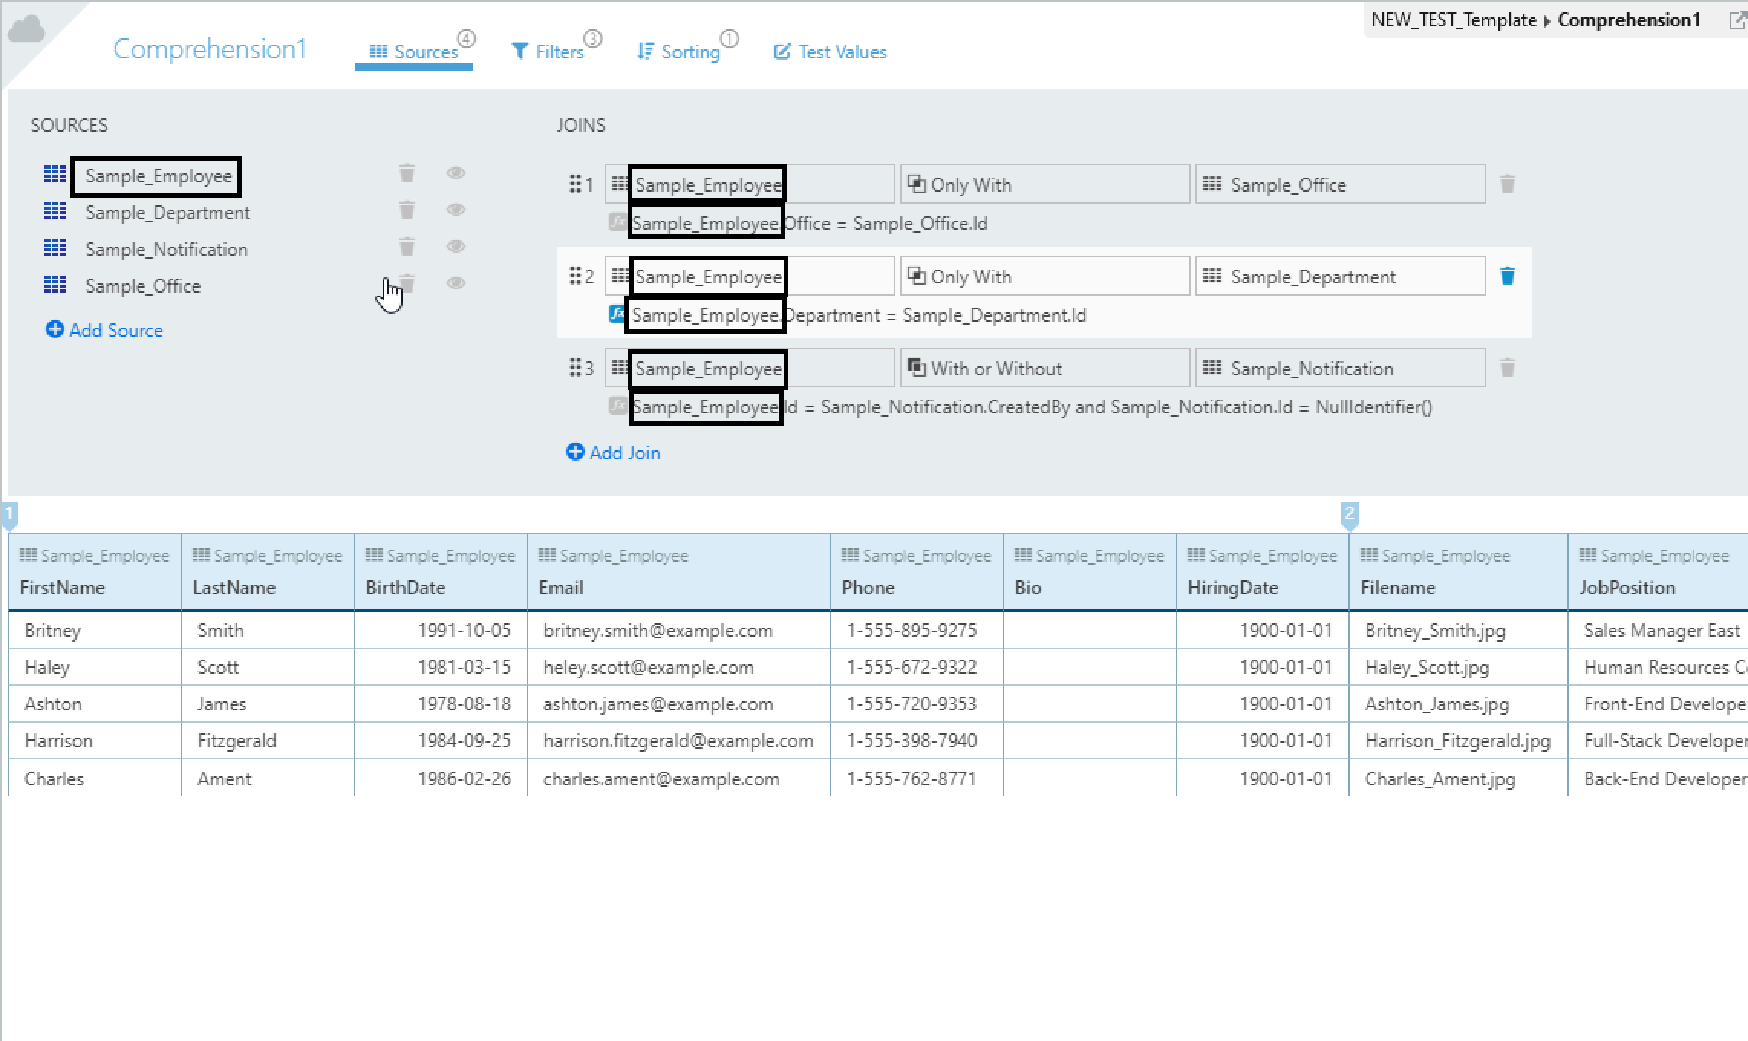
\includegraphics[height=2.7in]{example-textual-language-overloading}
	\caption{Example of the existing textual language overloading - The entity $"Sample\_Employee"$ is represented seven times. }
	\label{fig:exampleTextualLanguageOverloading}
\end{figure}

Therefore, the way entities and joins were listed in the sources tab of the existing interface was reconsidered, since it was intended to create a simpler, intuitive, and compact viewing area.

The idea of a tree view which displays all entities and joins used in the query has emerged to tackle the problem mentioned. Through that approach, it would be possible to reduce the entity repetition and to explicitly perceive which entities have a certain entity been joined.

\medskip

\textbf{Query formulation improvements: }

\medskip

%learnability
Regarding query formulation, there was several users who are not accustomed to the query builder, that had difficulty to discover some functionalities of the system when they tested the existing interface. Thereby, learnability was also considering during the design phase of the first prototype.

As mentioned in \ref{subsec:analysis}, the options to add a new calculated attribute or to apply a group by or an aggregation functions are hidden. These functionalities could be frequently used to apply group data or to add a new column to the output. Therefore, it was concluded that these options should be visible in the sources area. By doing this, not only the options still more visible to the novice users but users have a faster alternative to insert these query components.

%efficiency

Lastly, the distribution of the formulation options (i.e., the buttons or other interface elements that allow users to insert new elements in the query) in the screen was a relevant aspect considered. If the controls of a query component are

The main concern was to put these controls near to the area where the content will be displayed. As an example, if there is an area where entities, joins, and attributes are placed together, the related interaction should be accessible near them. In that way, users do not need to find options in other areas of the interface, keeping the user task on track, avoiding them to lose reasoning context.

That design principle was considered advantageous to reduce the user's working memory overload since they could focus in each part of the query without distractions. Moreover, if the controls are near the time the mouse need to move to them is also less, accelerating the query formulation process.

%Falar da divisão e distribuição do layout
%Falar que tendo em conta o espaço disponível seria necessário encurtar a representação das sources e joins.
%Adicionar fatores diferenciadores para a leitura da query: color highlighting nos filters, melhorar a leitura dos dados na tabela dos resultados, adicionar opções mais visíveis e acessíveis (práticas, rápidas) para adicionar novos attributos.

%Para além disso, foi mais tido em conta a preocupação de colocar numa sub região da interface a maior parte dos controlos mais utilizados, de modo a formulação da query poder ser realizada de forma mais rápida e eficaz, visto que não só se diminui o tempo através da menor distância que o rato tem que percorrer, como também porque o  utilizador vai mantendo o mesmo contexto visual.


\subsection{Implementation}
\label{subsec:paper_prototype_implementation}

After defining priorities for the current design iteration, the paper prototype implementation has launched. In this phase, the pieces of the prototype were built progressively considering the key points presented before and refining some details whenever necessary.

\medskip

\textbf{General layout:}

\medskip

As the reasoning applied in the design phase, the general layout was the first part implemented. The main concern at this phase was the definition of the dimensions for each sub-editor. In order to ensure that the design will be properly integrated into the Service Studio, it was created a sketched background image of the \gls{IDE} using a function of Balsamiq \cite{balsamiq} to convert the Service Studio screenshot to a black and white line drawing version \cite{balsamiq_using_images_and_assets}. As a result, it was possible to perceive if the design done would combine with the system where its is integrated without increasing the fidelity level of the prototype.

After that, the main areas of the interface were elaborated until reaching the general layout that can be observed in Figure \ref{fig:paperPrototypeGeneralLayout}.

\begin{figure}[htbp]
	\centering
	\includegraphics[height=3.0in]{paper-prototype-general-layout}
	\caption{Paper Prototype general layout.}
	\label{fig:paperPrototypeGeneralLayout}
\end{figure}

\medskip

\textbf{Query Result Table:}

\medskip

The next step was the design of the query result tables necessary to show the result preview of the query built. It was designed tables for all user testing scenarios to provide a real context to users when they tested the prototype. 

In order to accelerate the process of the table design in paper, it was used the same Balsamiq functionality used fro background to transform the table of the existing interface into a low-fidelity design. 

However, the headers of the table were redesigned manually to improve the readability of the table. Basically, in the existing table, the user needs to apply more effort to understand where start the data from an entity and where there is data from another entity. In that way, the entity reference in table header were merged to give to the user an easier perception that all the attributes below belong to the entity above. Figure \ref{fig:queryResultTableComparison} compares the existing one to an example of one of the tables built.

\begin{figure}[tb]
  \centering
  \subcaptionbox{Existing Interface\label{fig:queryResultTableComparisonExisting}}%
    {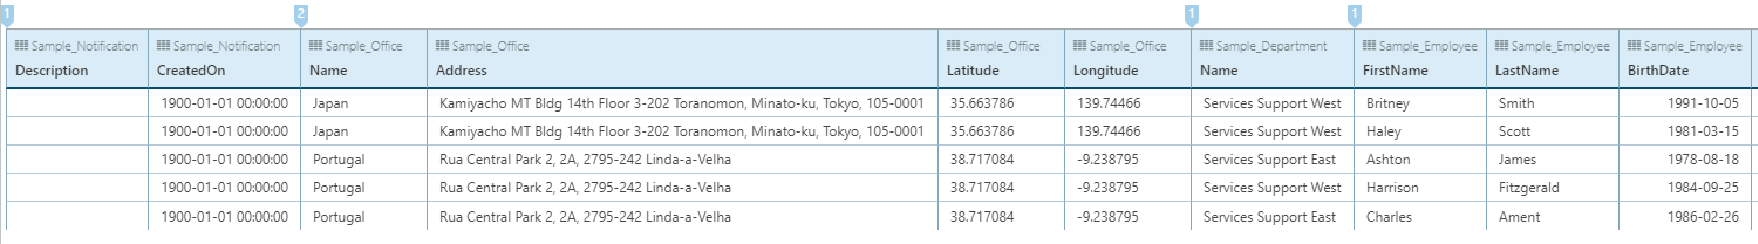
\includegraphics[width=0.9\linewidth]{query-result-table-existing}}%
    \\
  \subcaptionbox{Paper Prototype\label{fig:queryResultTableComparisonPaper}}%
  {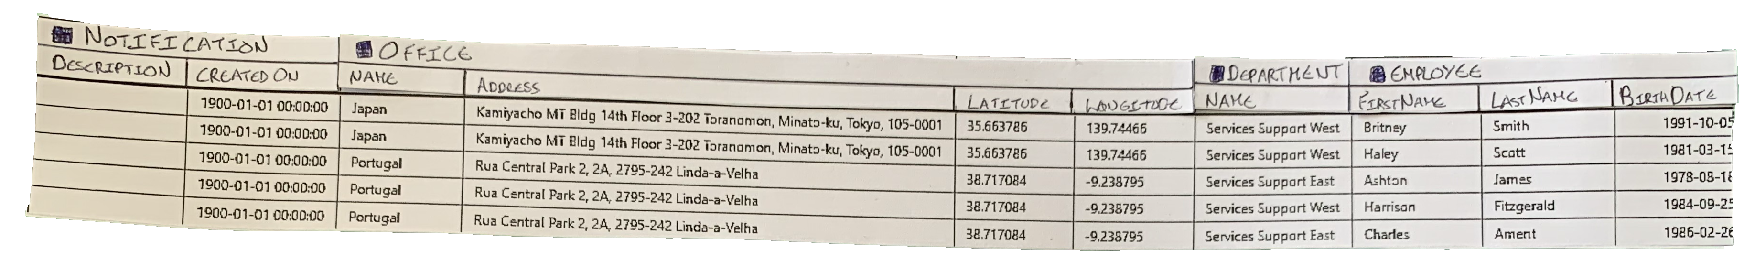
\includegraphics[width=0.9\linewidth]{query-result-table-paper}}%
\caption{Comparison between the existing query result table and the designed for the Paper Prototype.}
  \label{fig:queryResultTableComparison}
\end{figure}

\medskip

\textbf{Filters and Sorting: }

\medskip

Regarding filters and sorting, it was decided to not apply major changes since there were other problems considered as most relevant. Even though the filters edition could be faster using accelerators such as copy and paste or the possibility to edit each filter in line instead of opening always the expression editor, these problems as well as other similar problems mentioned in the Appendix \ref{app:taxonomy_of_problems_existing_interface} - \nameref{app:taxonomy_of_problems_existing_interface} were not tackled. The reason to disconsider these improvements in the prototyping phase was that there are straighforward improvements that have a low-risk associated since they might not affect negativle the user's experience. That way, it was given focus to the designs parts that should be rigorously tested by users to ensure that riskier changes are improving the usability of the interface.

Accordingly, concerning filters, it was only added some syntax highlighting to each one of the conditions presented in order to reduce the time required to understand the conditions. Figure \ref{fig:filtersAndSortingComparison} presents an example of Filters and Sorting design in the paper prototype.

\begin{figure}[tb]
  \centering
  \subcaptionbox{Existing Interface\label{fig:filtersAndSortingExisting}}%
    {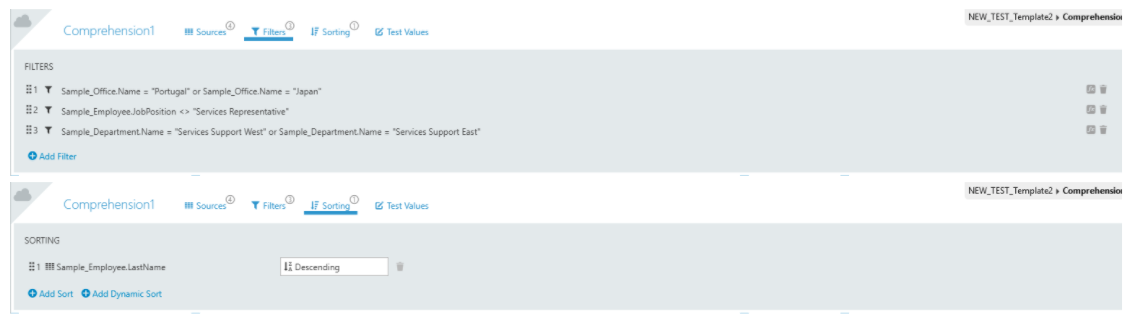
\includegraphics[width=0.9\linewidth]{existing-filters-sorting}}%
    \\
  \subcaptionbox{Paper Prototype\label{fig:filtersAndSortingPaper}}%
  {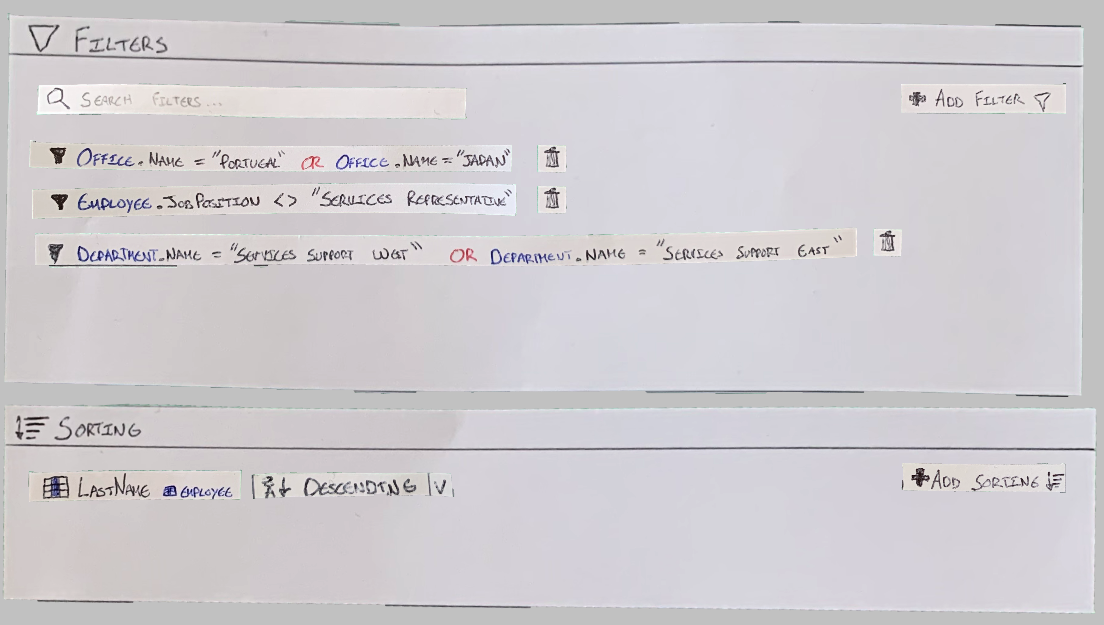
\includegraphics[width=0.9\linewidth]{paper-filters-sorting}}%
\caption{Comparison between the existing filters and sorting sub-editors and the ones designed for the Paper Prototype.}
  \label{fig:filtersAndSortingComparison}
\end{figure}

\medskip

\textbf{Sources View: }

\medskip

As referred before, the design of the sources view was considered one of the most impactful aspects to improve the query builder usability. The restructuration design of this element was reasoned as a crutial section of the interface that could leverge the usability of the system. 

A new approach to represent sources and joins was built progressively. The first aspect approached was the creation of a hierarquical view similar to a tree view which gives to the user the perception of what entities are related with each other. Figure \ref{fig:simpleSourcesTree} shown an example of a tree built at that stage.

\begin{figure}[htbp]
	\centering
	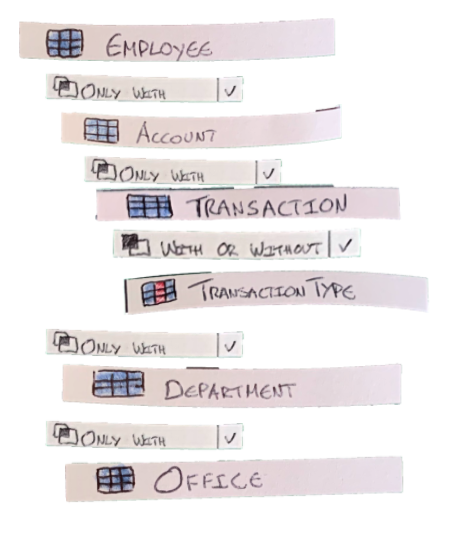
\includegraphics[height=2.7in]{simple-sources-tree}
	\caption{First stage of the design of a new representation approach to display sources and joins.}
	\label{fig:simpleSourcesTree}
\end{figure}

Notwithstanding the visual simplicity achieved, that representation is insufficient since it not represents the join conditions. However, if join conditions were just included near to the join type, the interface would be overloaded again and it would still poor readability.

Furthermore, the usability tests of the existing interface have revealed that often users tended to misunderstand the queries that had joins with specific characteristics. In particular, in cases where queries had joins with conditions that contained logical operators or when the join between the two tables could be done through different attributes.

Through practical examples it is easier to understand the dimension of the problem. For example, considering the data model presented in Figure \ref{fig:dataModel}, if a user wants to query the employees and their departments, he will add the two entities and the visual query builder will build automatically the join condition:

\begin{center}
  \verb|"Sample_Employee.Office = Sample_Office.Id"|
\end{center}

This automatism is useful and turns the query formulation process more simple and efficient. However, there are cases where the join needs to be specified as the case is no so straighforward. For instance, considering the same data model, if a user wants to query the employees who are owners of accounts, the join condition has to merge the two entities $"Sample\_Employee"$ and $"Sample\_Account"$ using the foreign key $"Owner"$ and not the two other availables: $"CreatedBy"$ and $"Manager"$. In this case the condition required to build this query is:

\begin{center}
  \verb|"Sample_Employee.Id = Sample_Account.Owner"|
\end{center}

In these cases, the join condition, which in many cases is not so important as just covers the general case and it was generated automatically by the system, represents an important aspect of the query. However, as illustrated in the example of Figure \ref{fig:comprehension2JoinsExisting}, the existing interface represents all joins equally.

\begin{figure}[htbp]
	\centering
	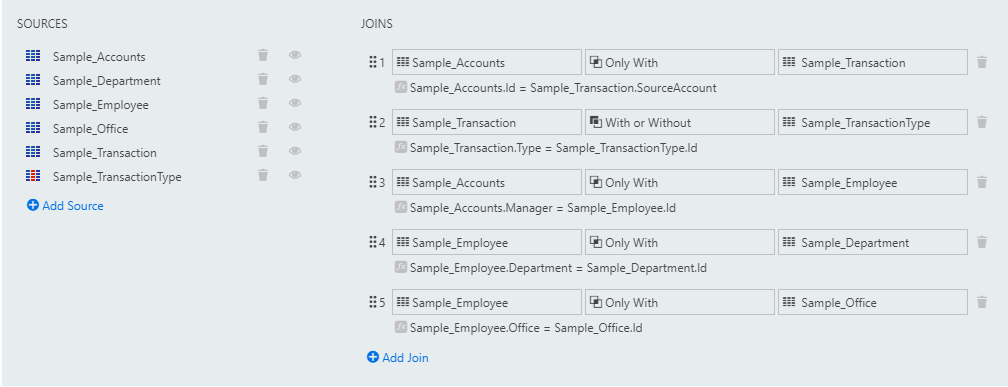
\includegraphics[height=2.2in]{comprehension-2-joins-existing}
	\caption{Example of joins representation in the existing interface in a query where the foreign key used to join is an important detail.}
	\label{fig:comprehension2JoinsExisting}
\end{figure}

When users tested the existing interface with cases similar to the one presented, two relevant usability problems were detected. On the one hand, when users tried to comprehend the query, most of them did not pay attention to this detail, not mentioning the foreign keys used. On the other hand, when they need to formulate queries that contemplates these cases, several users, even the most experienced using this query builder, did not select the intended foreign key. This behavior is normal since the system just assume one of the foreign keys and generate the join, without asking user what attribute he wants to use to join the two entities.

Therefore, the exploration of a new sources and joins representation was an excellent opportunity to tackle this problem. In that way, the existing tree view of sources was rebuilt in order to integrate also the foreign key used to build each of the presented joins. Moreover, when two entities are added and the join between them can be done through different keys, the system starts asking the user which key he wants to use. Figure \ref{fig:paperFkSelect} illustrates how this idea was transposed to the paper prototype.

\begin{figure}[htbp]
	\centering
  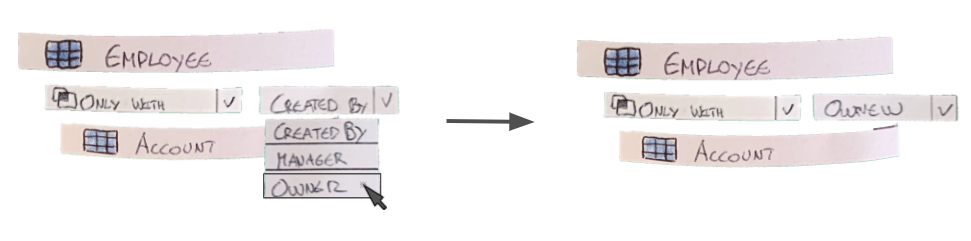
\includegraphics[height=1.4in]{paper-fk-selection}
	\caption{Example of the new foreign key selection and representation applied in the Paper Prototype.}
	\label{fig:paperFkSelect}
\end{figure}

Nevertheless, the foreign key is not the only aspect that could be specified in the join condition. As in SQL, the existing query builder allows user to edit manually the join condition, for example to add more restrictions using logical operators.

In these cases, not only is it important to continue to allow the conditions editing in the new interface but the conditions already edited should also be highlighted in such a way that users who open the query for the first time perceive that the condition of these joins is different. 

The strategy applied in the paper prototype to maintain the interface simple, clear, and intuitive while highlighting the relevant aspects was to put only the function icon in the simple join conditions, and the other ones has their difference explicitly represented after. Figure \ref{fig:paperComprehension1Sources} represents the sources of a query with a join condition edited. In this case the join condition between $"Sample\_Employee"$ and $"Sample\_Notification"$ was changed since the goal is to fetch the employees who have never created notifications. Accordingly, a simplification took place to represent only the differentiating factor instead of the full condition which is:

\begin{center}
  \verb|"Sample_Employee.Id = Sample_Notification.CreatedBy and| 
  \\
  \verb|Sample_Notification.Id = NullIdentifier()"|
\end{center}

\begin{figure}[htbp]
	\centering
  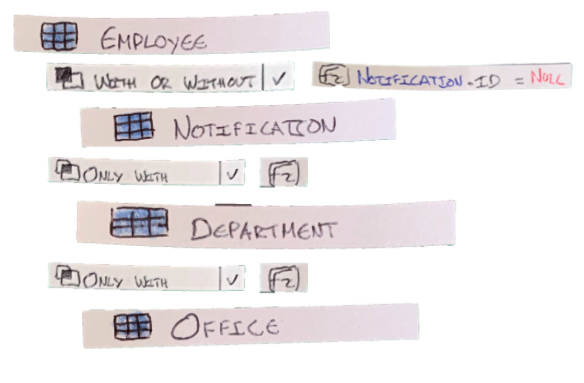
\includegraphics[height=1.4in]{paper-comprehension-1-sources}
	\caption{Example of the sources of a query that has a join with a condition edited.}
	\label{fig:paperComprehension1Sources}
\end{figure}

Through that approach, users will see entities and joins of the query without information overloading which could allow them to perceive easily and faster the purpose of the query. Even if the join condition is hidden, they could click on the function icon and an expression editor will appear where it is possible to see and edit the join condition selected.

\medskip

\textbf{New alternatives to add and search for attributes:}

\medskip

The last improved aspect during the development of this paper prototype was regarding the addition of new attributes. In accordance with the mentioned in the last section, there was a demand to provide other alternatives to add calculated attributes as well as group bys or aggregation functions.

Considering the concern to insert these alternatives strategically in easily and fast accessible places and the necessity to improve the visibility of these options to improve the learnability of novice users, the following options were applied:

\begin{itemize}
  \item \textbf{Click and right-click in the attributes exhibited in the Sources sub-editor: }The list of the attributes of each entity was added into each entity represented in the Sources of the query. On the one hand, if users click in an attribute, they would see the data related into the query result preview (according to the sketch already presented in Figure \ref{fig:sketchAttributeSearch}). On the other hand, if they right-click in an attribute, they would see the same context menu that they already could see when they right-click on the result table headers. Therefore they could apply operations using that alternative, as exemplified in Figure \ref{fig:paperAttributeRightClick}.
  \item \textbf{Two new visible buttons to add attributes: }In the footer of the Sources View, two buttons were added:
    \begin{itemize}
      \item \textbf{Aggregation / Group By: }Clicking in this button the user could choose an attribute and one of the following operations to group the data of its attribute: Group by, Sum, Average, Max, Min, or Count. Figure \ref{fig:paperAddAggregation} shows this new formulation area.
      \item \textbf{Calculated Attribute: }When the user selects this option the interface will show an expression edition area similar to the existing one to indicate the formula of the new attribute. Figure \ref{fig:paperAddCalculatedAttribute} shows this alternative to add a new calculated attribute.
    \end{itemize}
\end{itemize}


\begin{figure}[htbp]
	\centering
  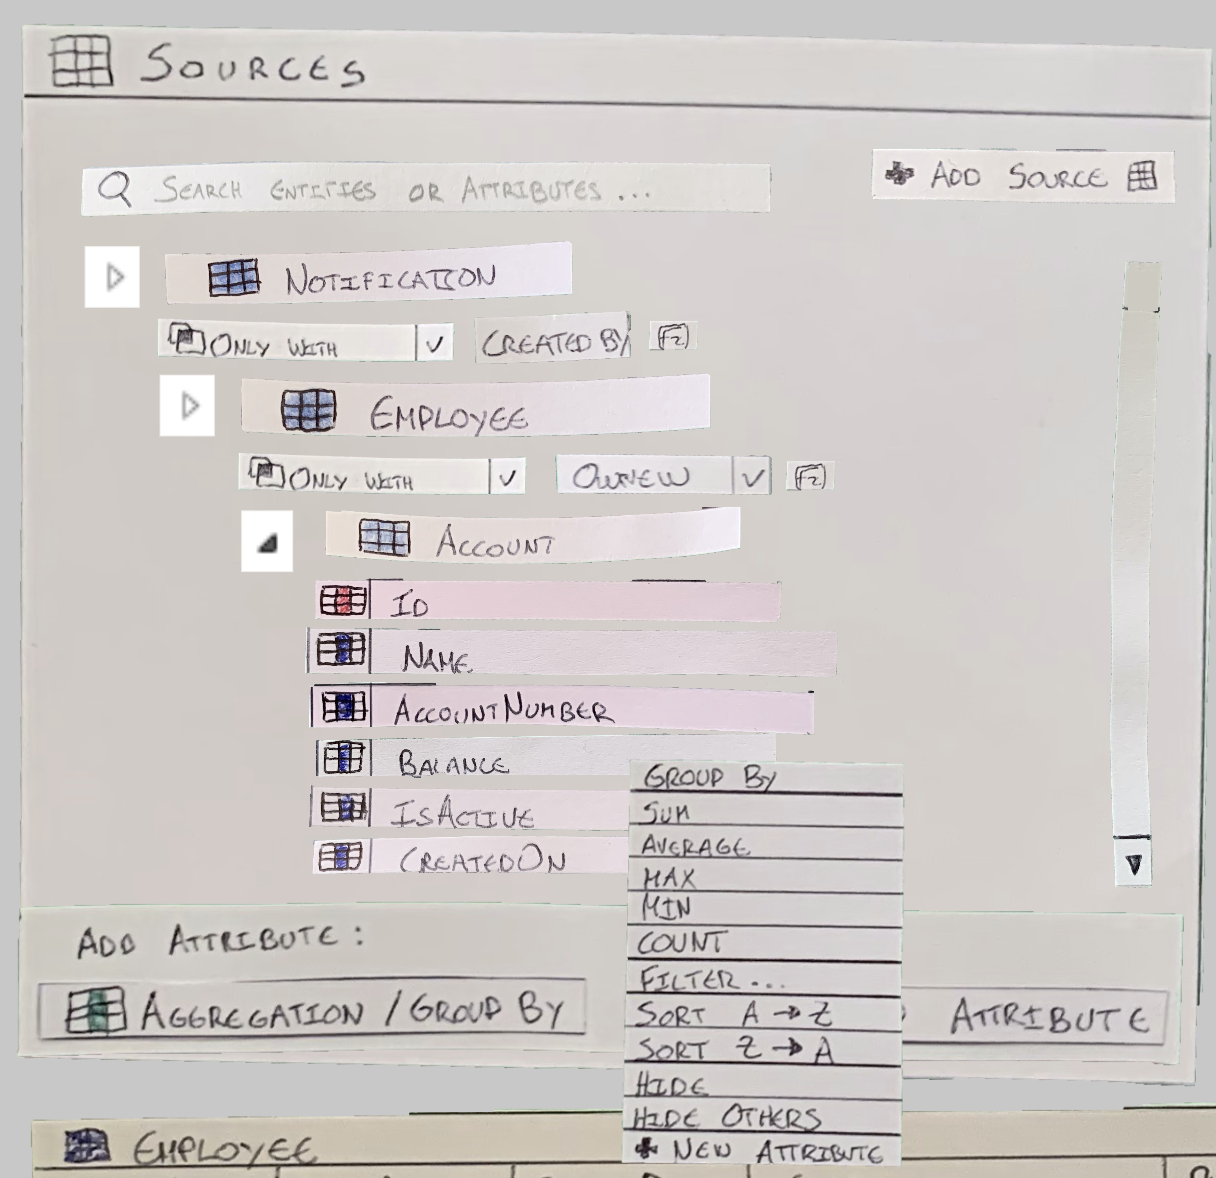
\includegraphics[height=2.4in]{paper-attribute-right-click}
	\caption{Alternative provided to open the attribute context menu.}
	\label{fig:paperAttributeRightClick}
\end{figure}

\begin{figure}[htbp]
	\centering
  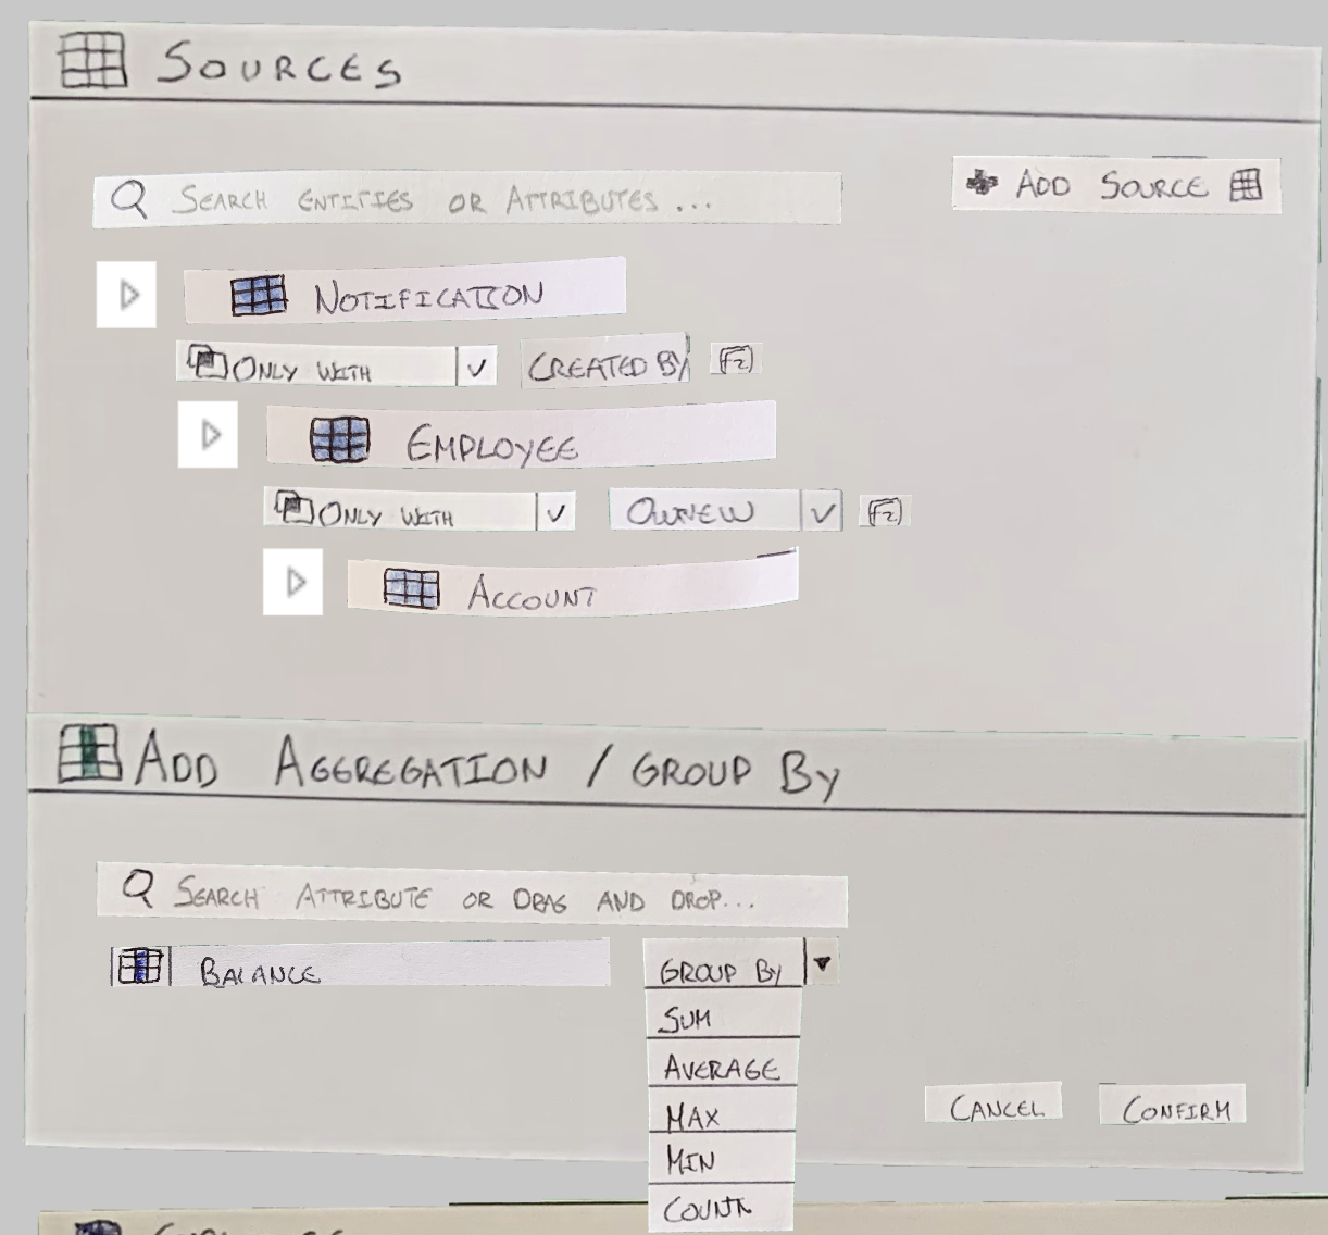
\includegraphics[height=2.4in]
  {paper-add-aggregation}
	\caption{New sub-editor into the sources view to add aggregation functions and group bys.}
	\label{fig:paperAddAggregation}
\end{figure}

\begin{figure}[htbp]
	\centering
  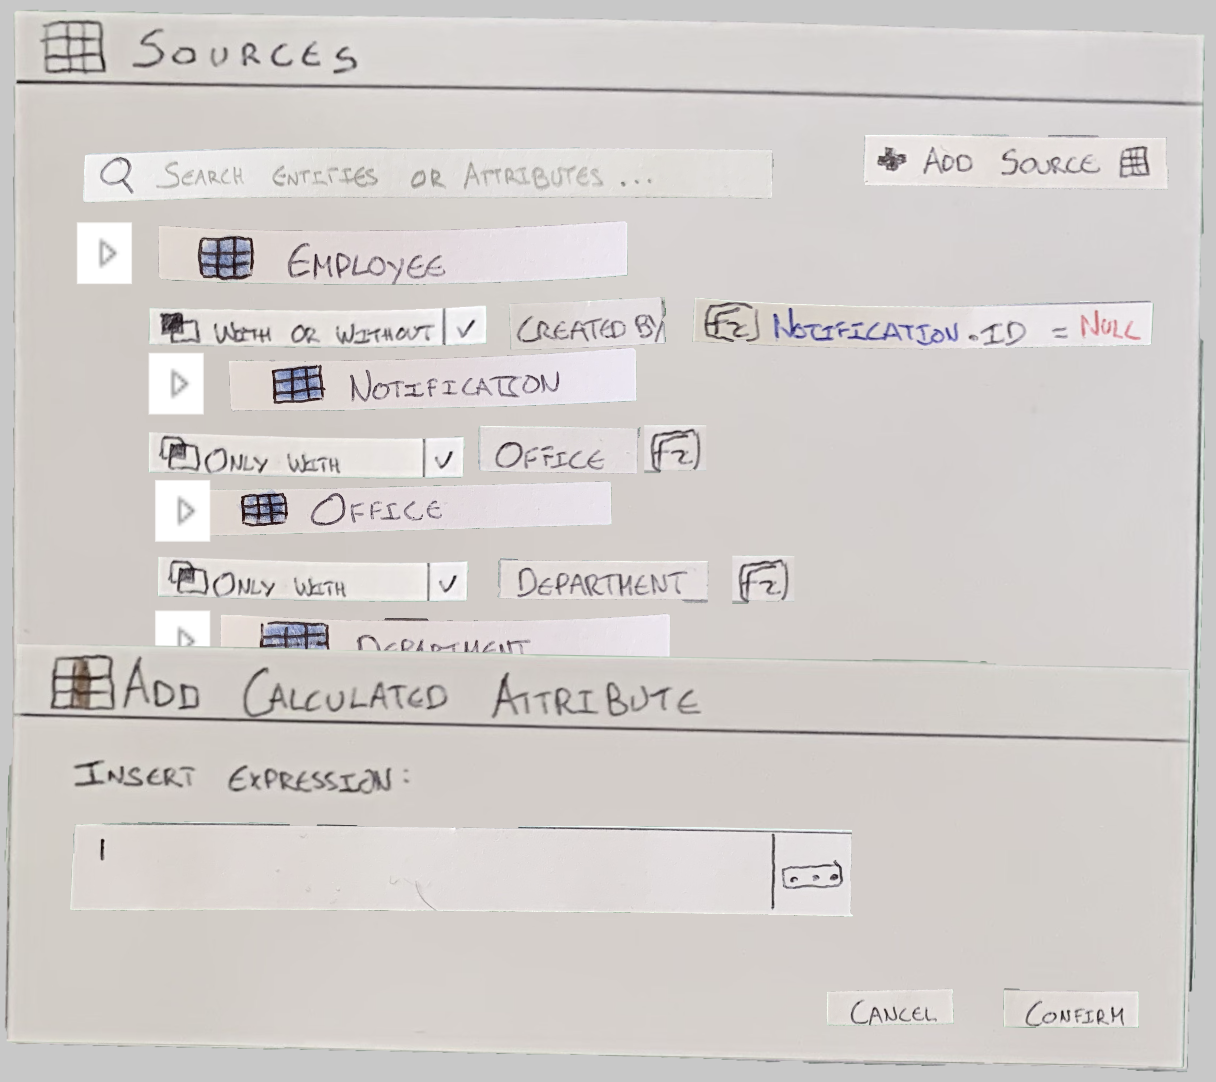
\includegraphics[height=2.4in]
  {paper-add-calculated-attribute}
	\caption{New sub-editor into the sources view to add calculated attributes.}
	\label{fig:paperAddCalculatedAttribute}
\end{figure}

In order to improve the query readability and the consistency of the interface, these attributes, added to the query, were put into the sources view as exemplified in Figure \ref{fig:paperAggregatedAttribute}.

\begin{figure}[htbp]
	\centering
  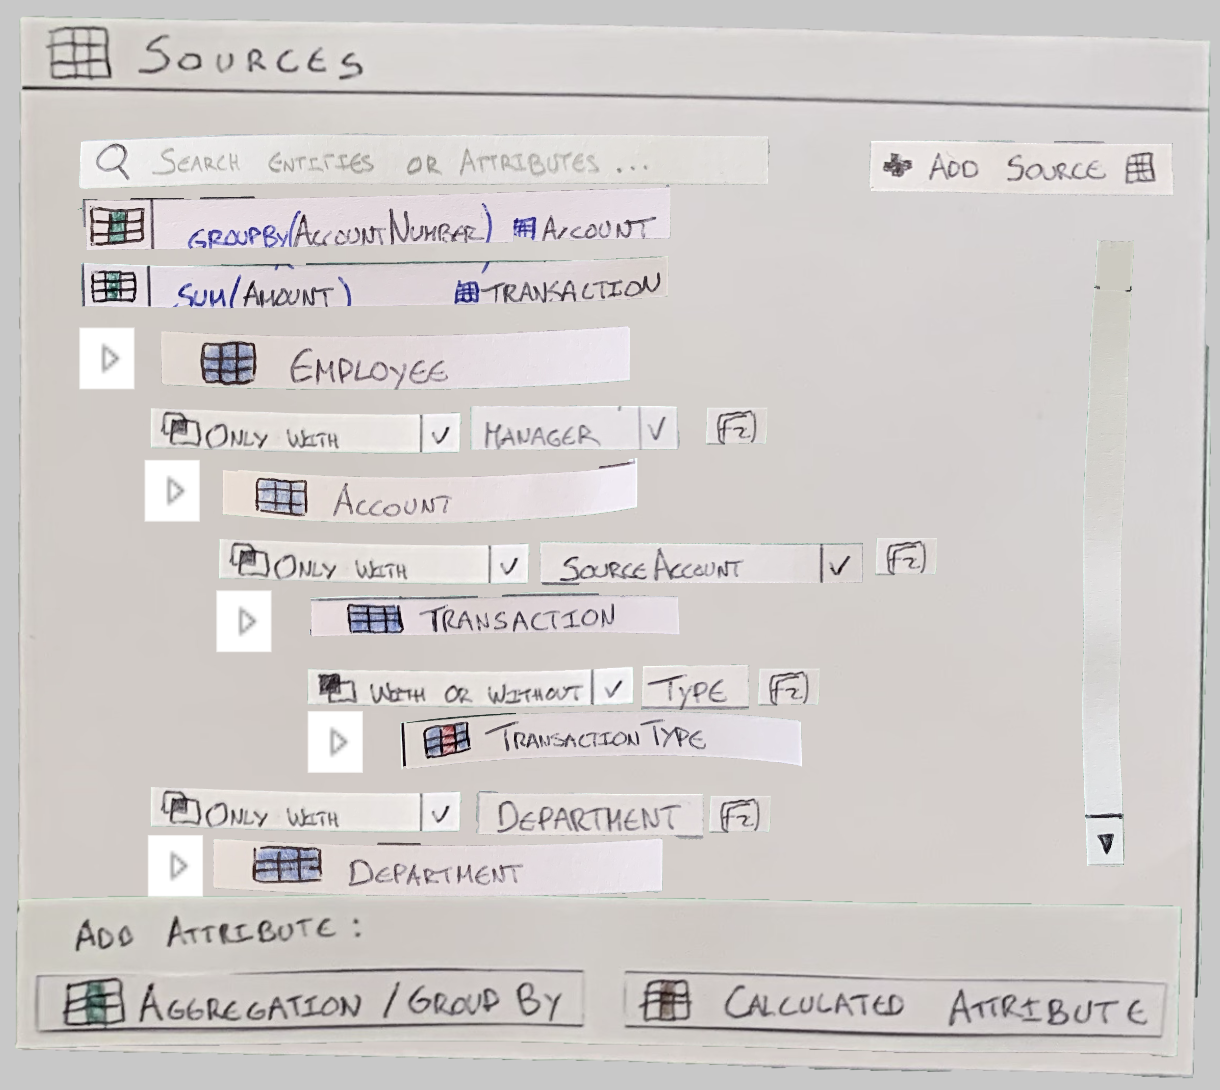
\includegraphics[height=2.4in]
  {paper-aggregated-attribute}
	\caption{Sources of a query where a group by and a SUM aggregation function were applied.}
	\label{fig:paperAggregatedAttribute}
\end{figure}

\medskip

\textbf{Digital Paper Prototype: }

\medskip

Combining all the components elaborated in paper, the result is illustrated in Figure \ref{fig:paperPrototypeExample}. In order to make it testable remotely, each one of the interface components were scanned and composed again using the InVision App \cite{invision}.

\begin{figure}[htbp]
	\centering
  \includegraphics[height=3.2in]
  {paper-prototype-example}
	\caption{Final Paper Prototype before scanning it.}
	\label{fig:paperPrototypeExample}
\end{figure}

Therefore, for each scenario, it was required to build multiple images since each one represents a state among the interface manipulation. In that way, interactions were added to the components to configure the images sequence, as can be observed in Figure \ref{fig:invisionInteractionExample}.

\begin{figure}[htbp]
	\centering
  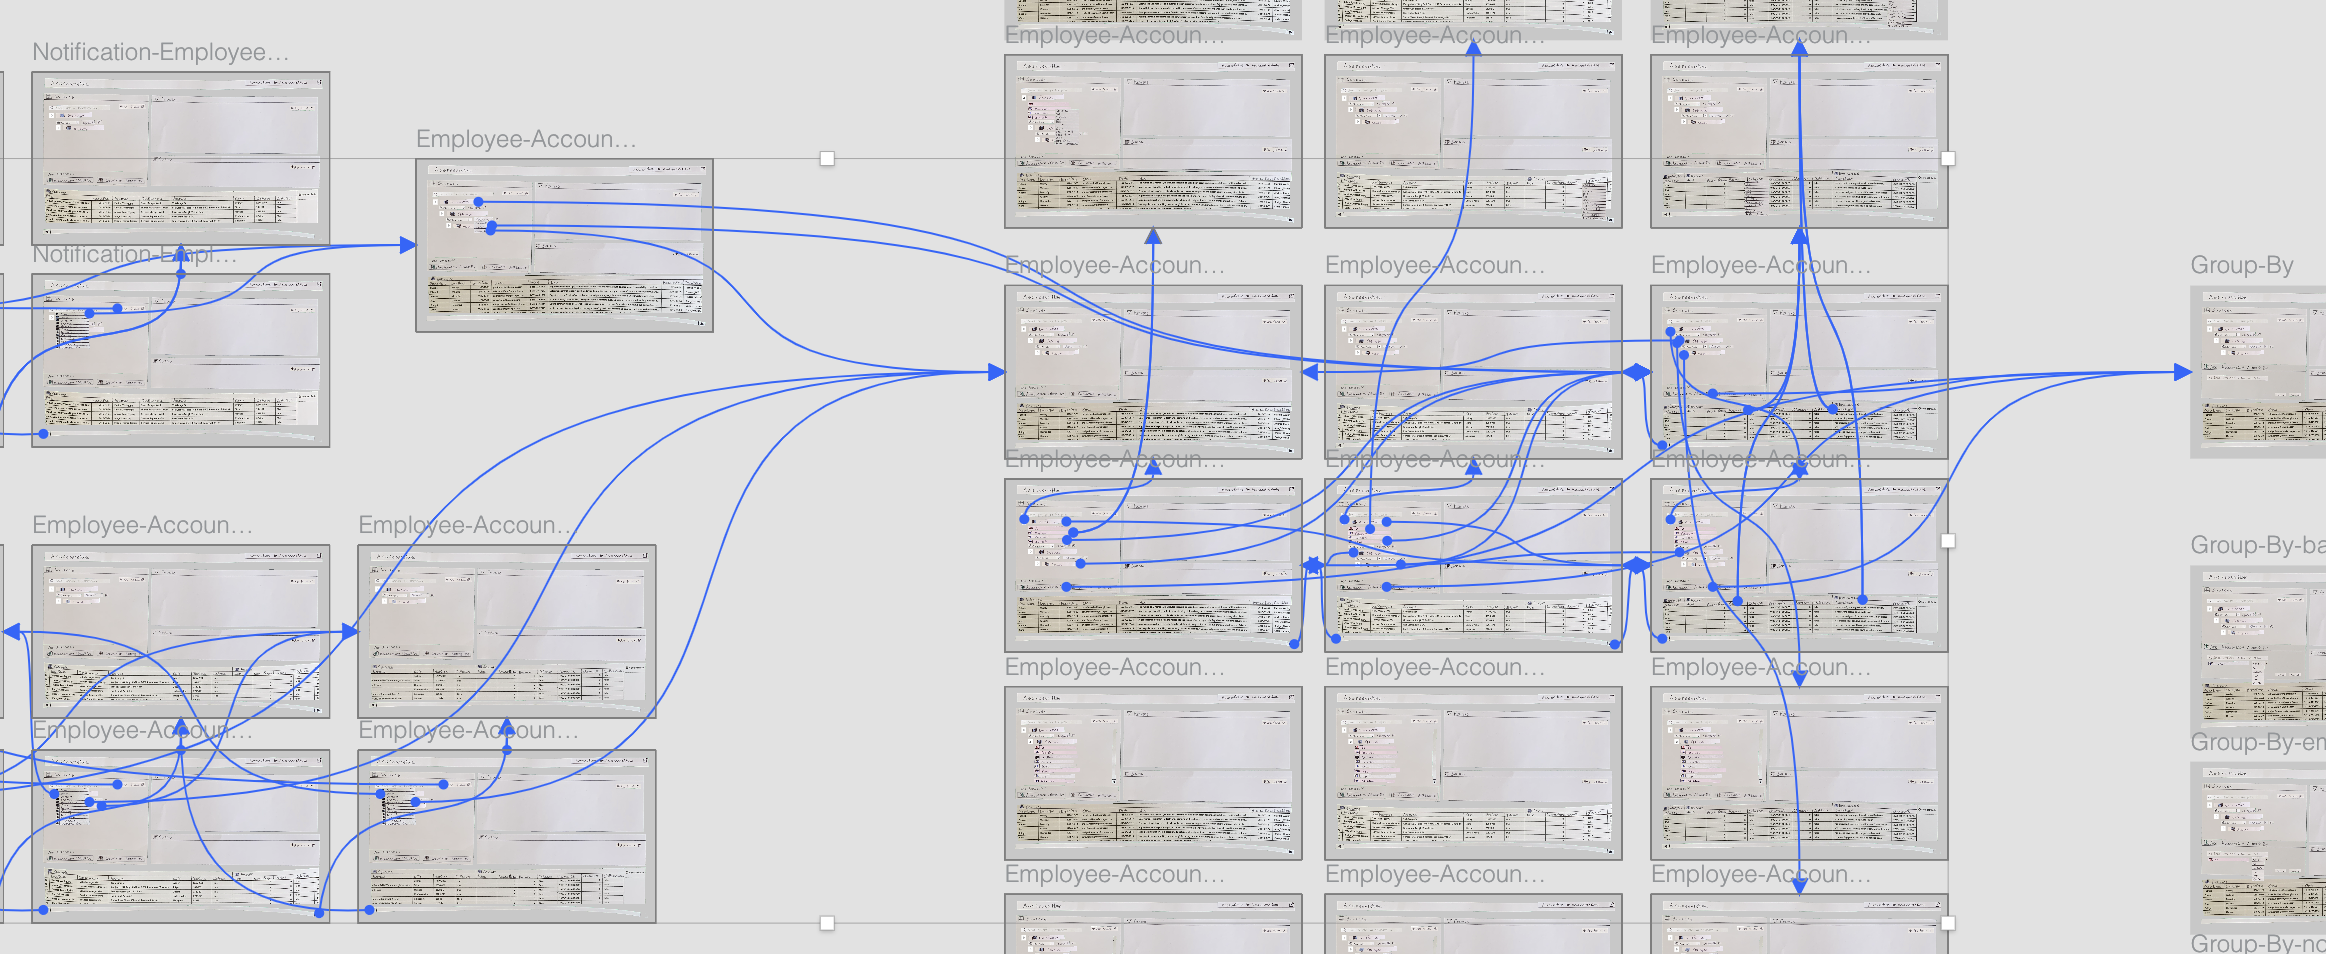
\includegraphics[height=2.4in]
  {invision-interaction-example}
	\caption{Brief example of the interaction configuration in InVision to turn the Paper Prototype testible in a fluid way.}
	\label{fig:invisionInteractionExample}
\end{figure}

In total, 291 images were created and multiple interactions between them were configured in order to reach a prototype that could be tested in all scenarios defined in the Appendix \ref{app:user_testing_scenarios} - \nameref{app:user_testing_scenarios} \cite{invision_managing_interactions}.

%Tabela do resultado para cada scenario
%Filtros e sorting de cada scenario

%New sources design
%-Falar sobre as chaves estrangeiras e a simplificação dos joins
%-Novas formas the inserir atributos
%-Apresentar solução proposta

% It is important to refer the implementation complexity of the prototype in InVision due to the interface complexity.

\subsection{Evaluation}
\label{subsec:paper_prototype_evaluation}

Completed the implementation of the Paper Prototype, the user testing phase has started. As mentioned in \ref{sec:iterative_design}, this prototype was tested with 5 users of each user group to perform a qualitative analysis regarding the changes applied in the interface. In that way, the aim, at this stage, was to map the improved aspects  and the details which require a redesign in the following phase.

In general, the new sub-editors layout applied was accepted positively by the users, even in the ones who were more accustomed to the previous tab layout. Although, at a first glance, some users claimed feeling overloaded with information, they mentioned, some minutes after, that see all query structure in a short visualization area above its result preview was useful. Other feedback pointed out by some users was that it could be useful to resize the dimensions of each sub-editor area.

%TODO: Colocar uma footnote para Background.currentProgress, onde existir uma imagem que demonstre como é que os group bys são atualmente representados.
Regarding the query result preview, some users did not manage to comprehend which attributes belong to the query output against the ones that were only a preview to understand the aggregations or group bys applied. Even though it was difficult to distinguish the two elements of the query result, since it was used a low-fidelity design which presented a low expressiveness in terms of color, this constraint will be taken into account in the next design iteration since more styling and color resources will be available.

As predicted in the design and implementation phases of this prototype, the completely redesigned sources editor evoked different points of view and interesting feedback for the next iteration design phase.

Therefore, the following points describe the information collected with respect to the users' comprehension of this new representation:

\begin{itemize}
  \item Some users misinterpreted the joins of some queries due to the indentation used to represent them. For instance, in the example shown in Figure \ref{fig:paperPrototypeExample}, some users indicated that "Office" was joined with "Department", when "Office" was joined with "Employee";
  \item Some users did not manage to understand what the foreign key label was, until they need to select one of them in the formulation scenario. That way, the representation of this element should be reevaluated to make it more clear;
  \item Regarding the join conditions simplification, it was identified an increased awareness to perceive that there were two representations of join conditions, as shown in Figure \ref{fig:paperComprehension1Sources}. However, the majority of users did not manage to understand the meaning of this different visual representation, which intended to differentiate joins automatically generated from the ones manually edited.
\end{itemize}

Furthermore, the following aspects were concluded from observing users trying to formulate queries:

\begin{itemize}
  \item As expected, the foreign key selection method presented in Figure \ref{fig:paperFkSelect} has optimized the effectiveness of the formulation scenario. Since users were asked to choose between the existing foreign key, they have selected the correct one.
  \item Concerning the two new buttons to add aggregation functions, group bys, and calculated attributes, it was concluded that, in part, the results have enhanced, but some drawback aspects were identified. Users who have never used the system, found these features easily since the two buttons became visible in the interface. However, they continue to make confusion when they needed to use a calculated attribute and an aggregation function.
\end{itemize}

Finally, some users referred that they felt a reduced necessity to confer the Data Model while they were building queries, since the new sources representation showed how entities were related with each other.

%Comparison with Current Implementation Evaluation

%Quantos utilizadores foram testados
%Dada a população utilizada só foram feitas análises qualitativas como meio de obter feedback construtivo para a próxima iteração.

%Explicar resultados mais importantes
%-Verificar os outros resultados
%-Melhoria da sources view visto que os utilizadores não perceberam que se tratava da chave estrangeira.
%Para além disso houve quem não achasse clara a apresentação devida à identação utilizada. (Por exemplo confundiram que tabela se relaciona com qual. Utilizar o exemplo do Comprehension 1 para justificar)

%-No geral o problema da leitura do left join com null manteve-se

%-Confundiram quando é que devia ser adicionado um calculated attribute e uma aggregation function.

%V-Alguns utilizadores referiram que o tamanho dos sub editores devia ser resizable

%-Divide add aggregation / group by into two different buttons

%-Some users said that the sources view is confusing at the first place but after some scenarios when he said that is easy.

%-Deveria ser apresentada uma maior distinção entre os atributos que estão no output e aqueles que não estão.

%-Tentaram expandir a source para adicionar joins.

%-Houve quem referisse que com esta interface existiu menos necessidade de observar o data  model

\section{Service Studio Implementation}
\label{sec:service_studio_implementation}

As mentioned in \ref{subsec:visual_development_environment}, the Service Studio is the \gls{IDE} integrated in the OutSystems Platform that allows users to build full applications using the low-code programming paradigm.

The last iteration of the design process, and consequently, the final prototype elaborated in this dissertation, was a functional prototype of the query builder completely integrated into the code of the Service Studio.

Nevertheless, Service Studio was getting a major facelift to achieve a new revamped and refreshed design. Even though the new Service Studio design was not been released yet when the development of the final prototype of this dissertation started, it was decided to start the development from this stage. In that way, the interface of the query builder developed could be easily integrated later on the OutSystems Platform. Figure \ref{fig:aggregateNewDesign} illustrates the design used as the starting point for the final prototype development. As can be observed, is a redesigned version of the previous Service Studio design illustrated before in Figures \ref{fig:ss_workspace} and \ref{fig:aggregate_created}.

\begin{figure}[htbp]
	\centering
  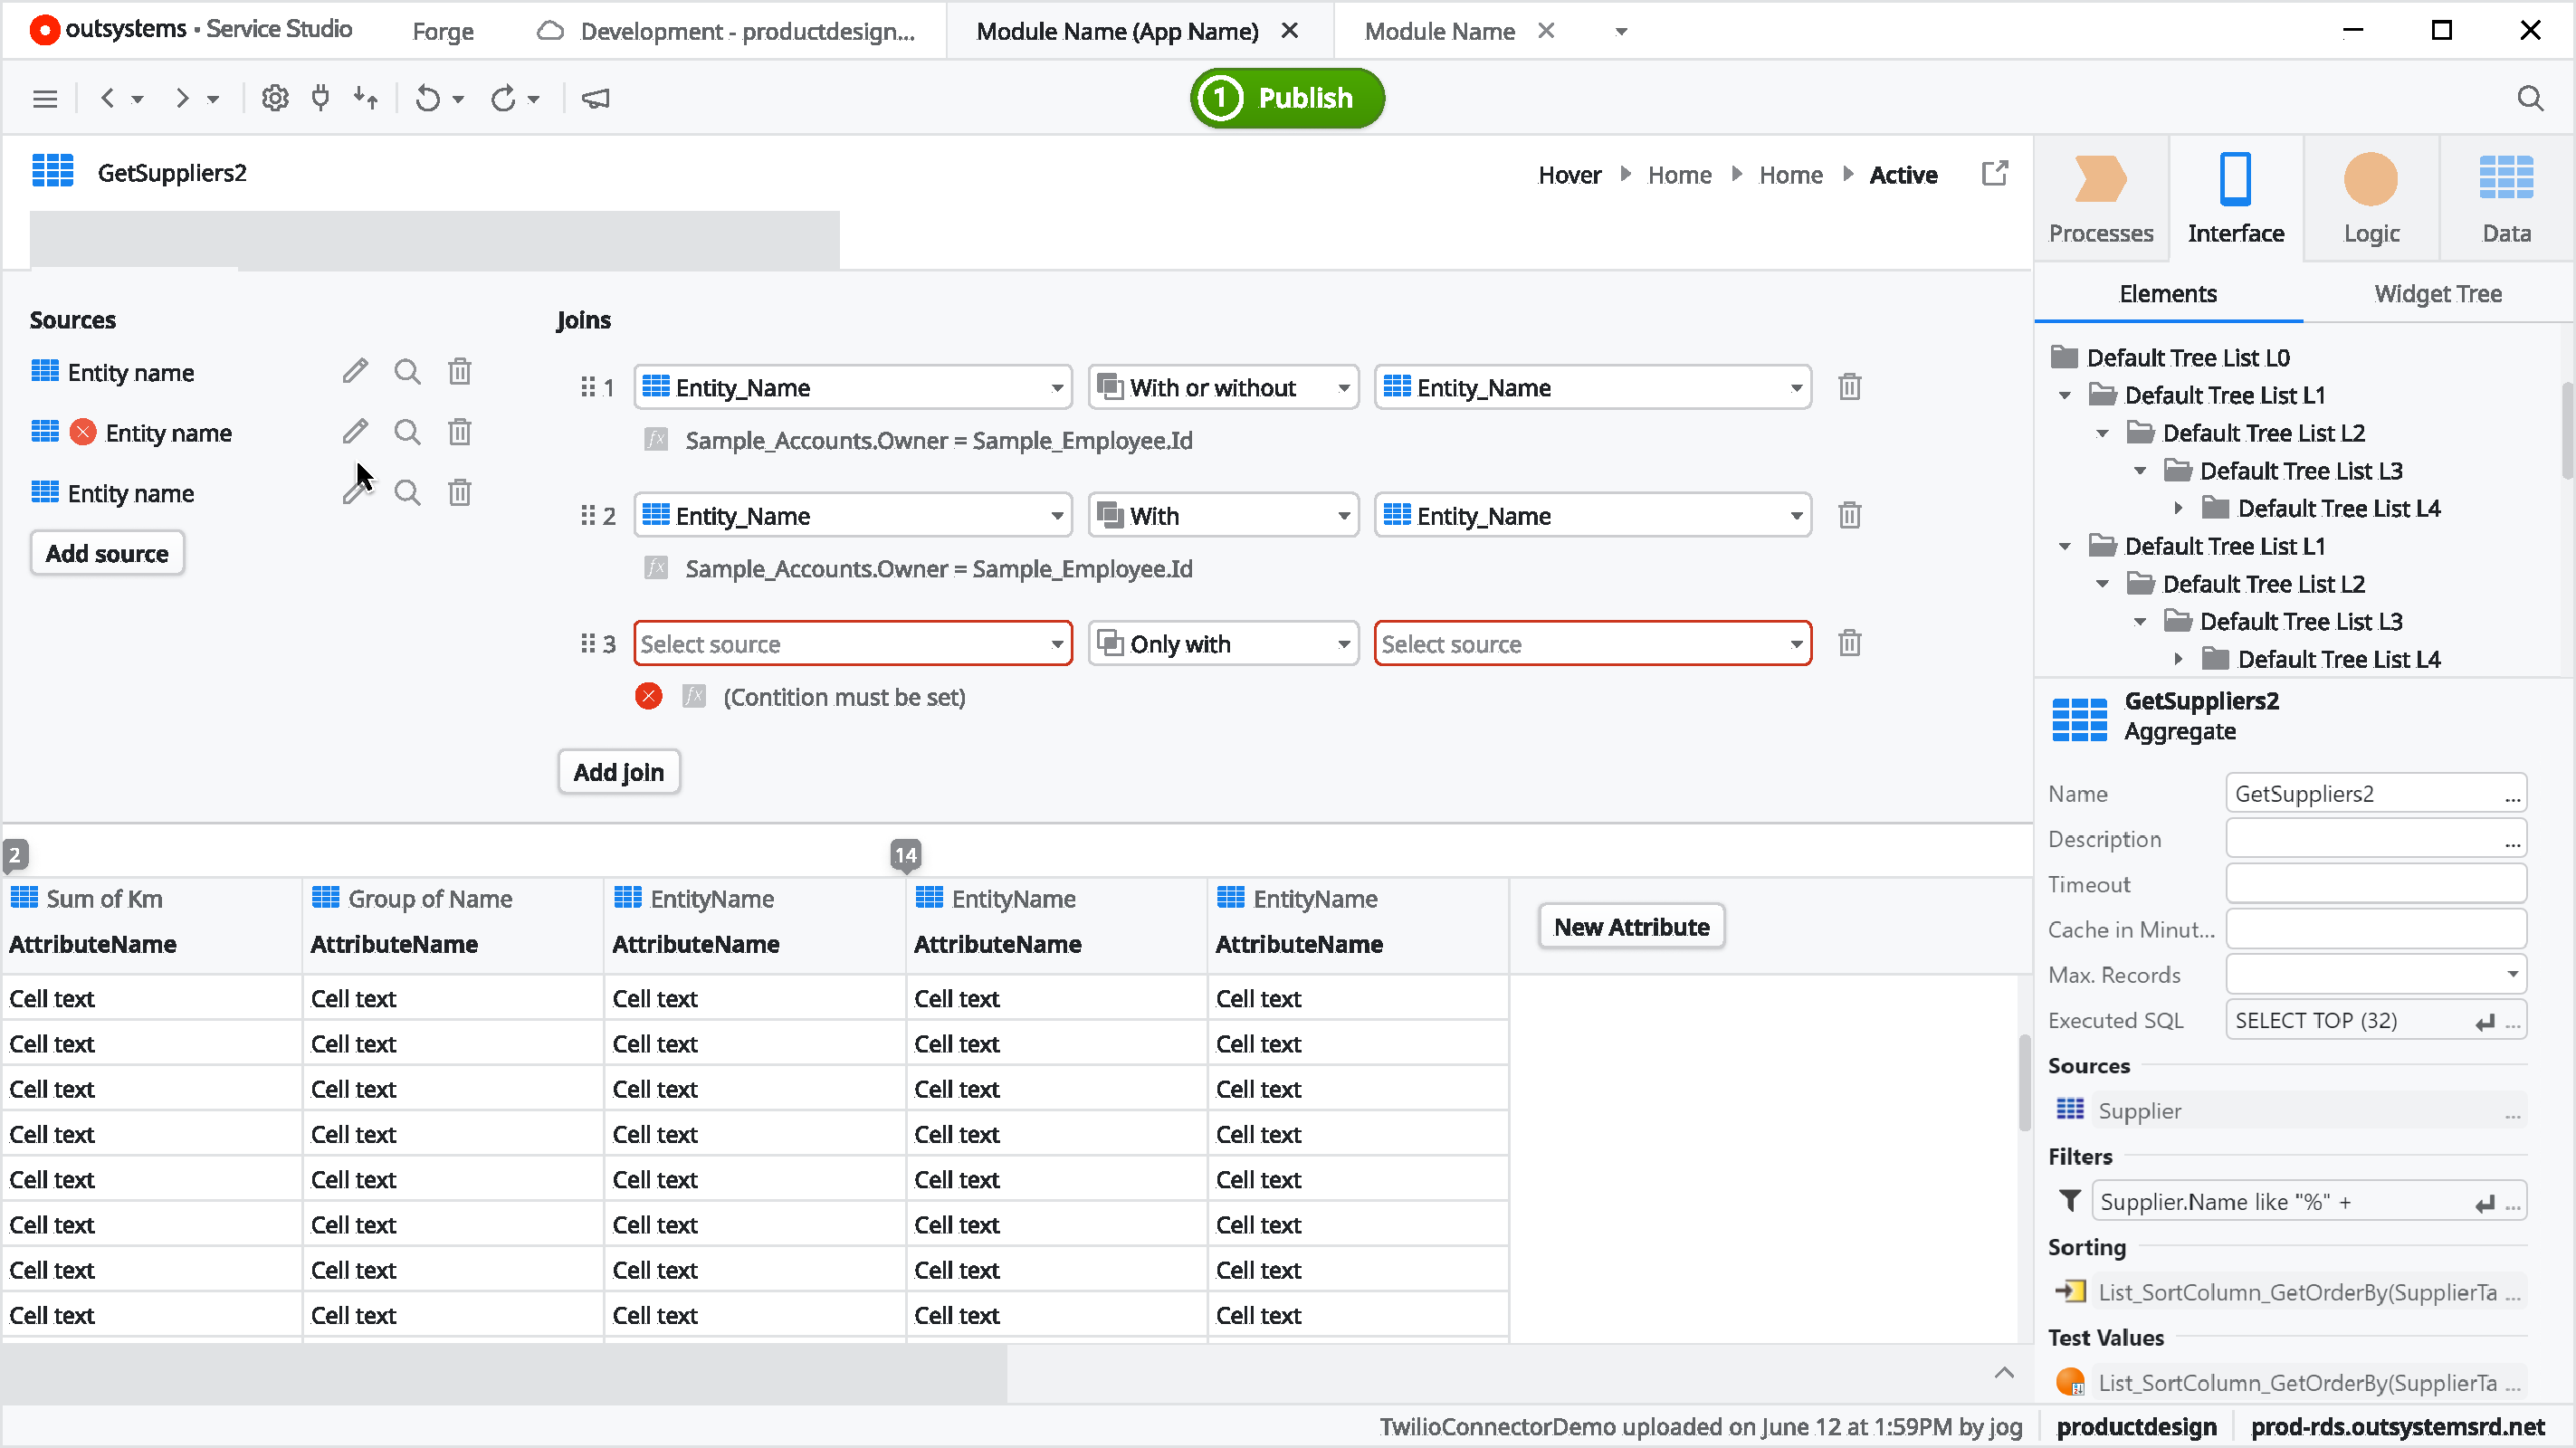
\includegraphics[height=3.0in]
  {aggregate-new-design}
	\caption{The new design of the Service Studio and its Visual Query Builder.}
	\label{fig:aggregateNewDesign}
\end{figure}

Despite the new design of all interface elements and components, the core behaviors and interactions of the interface remained, so the same design and implementation intentions to be applied in this new phase of development were maintained.

\subsection{Design}
\label{subsec:service_studio_design}

Following the same methodology used in the Paper Prototype, the building process of this solution started with the design phase. In this phase, the paper prototype evaluation outcomes were deliberated in order to define and prioritize the aspects to be tackled in the final prototype.

First of all, the source code of the Service Studio was explored in order to plan the development that could be done in the time available. As explained in the presentation of the paper prototype, the development aspects were planned according to their impact on the final interface. Ideas that fundamentaly alter the experience of using the interface will be considered a priority, since the most important is to perceive how users reacted to that changes, when testing the interface. Minor features and enhancements could also be considered as future work if the interface evaluated had positive results.

Considering the performed evaluation of the Paper Prototype, the sources editor was taken into account as the main focus of the design phase of the Final Prototype. As referred, during the usability tests of the paper prototype, the sources view has revealed positive results, but it was concluded that it should be refined regarding some aspects, mainly the joins representation which were not completely clear for a set of users.

Nevertheless, in order to implement the new interface representation of entities and joins, a considerable implementation effort would be required. The visualization area requires a personalized hierarquical view that should be built from scratch, since there is no similar element in the rest of the Service Studio.

Accordingly, before implementing any idea, a robust design should be established in order to avoid wasting implementation time on doing and redoing ideas. Therefore, it was performed more designs, regarding this region of the interface, using the product design system components. Basically, it was used the Figma \ cite {figma}, which is a design tool where all the new Service Studio components were designed, to explore concrete options to represent sources and solve the problems found when users tested the Paper Prototype. By this means, it was possible to obtain an high-fidelity design faster and perceive what solution could most fit the existing requirements.

After exploring multiple alternatives, the options illustrated in Figure \ref{fig:sourcesFigma} were considered the most valuable. The main difference between them is the way the joins are represented. In \nameref{fig:sourcesFigmaA}, the join is represented in a single line placed between the two entities involved. In \nameref{fig:sourcesFigmaB}, the join condition is represented after the the second entity involved in the join. Lastly, in \nameref{fig:sourcesFigmaC}, the second entity is presented on the right of the join kind.

\begin{figure}[tb]
  \centering
  \subcaptionbox{Option A\label{fig:sourcesFigmaA}}%
    {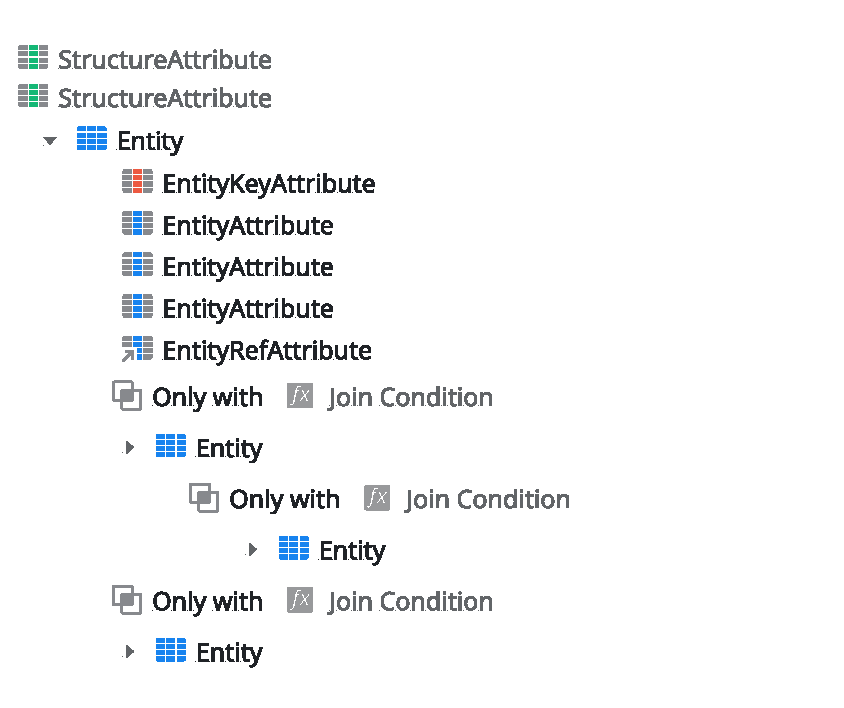
\includegraphics[height=2.5in]{sources-figma-1}}%
  \subcaptionbox{Option B\label{fig:sourcesFigmaB}}%
    {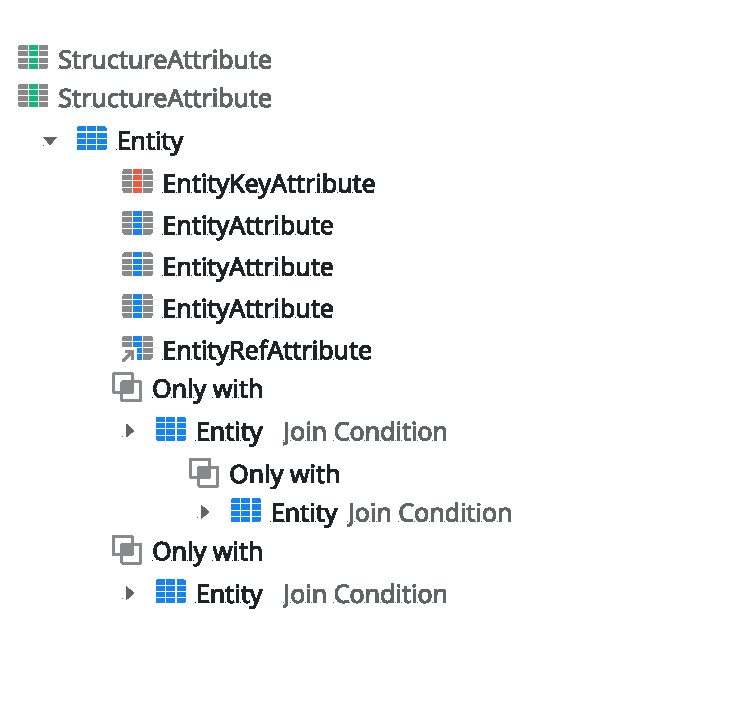
\includegraphics[height=2.5in]{sources-figma-2}}%
    \\
  \subcaptionbox{Option C\label{fig:sourcesFigmaC}}%
  {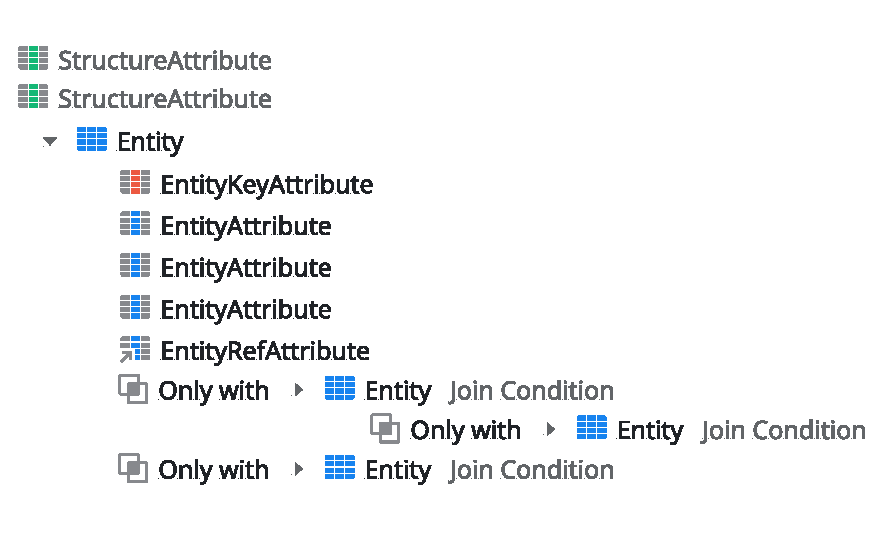
\includegraphics[width=0.5\linewidth]{sources-figma-3}}%
\caption{High-fidelity design ideas built in Figma to present the sources of the query.}
  \label{fig:sourcesFigma}
\end{figure}

In order to decide an option the following topics were taken into account:

\begin{itemize}
  \item \textbf{Reading flow: } The reading flow of the entities and joins were considered important, especially due to the presentation of the join kind. As this was presented in natural language, users should manage to read  sequentially the first entity, the join, and the second entity in a fluid way. Due to the arrangement adopted, the \nameref{fig:sourcesFigmaC} was considered the most clear regarding this aspect since the second entity is placed in the right side of the join kind. In that way, the users reading affordance will unconsciously help them to understand the reading flow, according to the reading pattern from the left to the right;
  \item \textbf{Width and height required: }The space each option would occupy was important to analyze the accommodation in the interface. Comparing the options presented, it can be concluded that the \nameref{fig:sourcesFigmaA} and \nameref{sub@fig:sourcesFigmaB} would require more height, and the \nameref{fig:sourcesFigmaC} more width;
  \item \textbf{Emphasis: }The used representation may end up giving more prominence to certain elements even though if it was not built for this purpose. Accordingly, it was verified the aspects of the interface which would stand out at a first glance. In \nameref{sub@fig:sourcesFigmaA} and \nameref{sub@fig:sourcesFigmaB}, joins are more highlighted since there are specific lines to represent them. Conversely, in the \nameref{sub@fig:sourcesFigmaC} the join is presented in the same line of an entity, which makes entities standed out, in general. Therefore, the \nameref{sub@fig:sourcesFigmaC} was considered the most appropriated to highlight entities at a first sight.
\end{itemize}

Reflecting on the topics presented, and evaluating the advantages and disadvantages of each option, the \nameref{fig:sourcesFigmaC} was elected since it provide a clear readability and highlights the entities used in the query. Despite it requires more width space in the interface, mainly if there are multiple joins nested, this disadvantages could be mitigated in the future if the join conditions would be simplified or represented in a different way.

Regarding the remaining elements of the interface, the design approaches applied in the Paper Prototype improved the usability of the interface. As a result, the design concerning filters, sorting and the query result table have followed the ideas already detailed in \ref{sec:paper_prototype}.


\subsection{Implementation}
\label{subsec:service_studio_implementation}
Having defined the intended design of the final prototype, the development of this new data querying interface integrated in the Service Studio code started. %As mentioned, the code is implemented in

\begin{figure}[htbp]
	\centering
  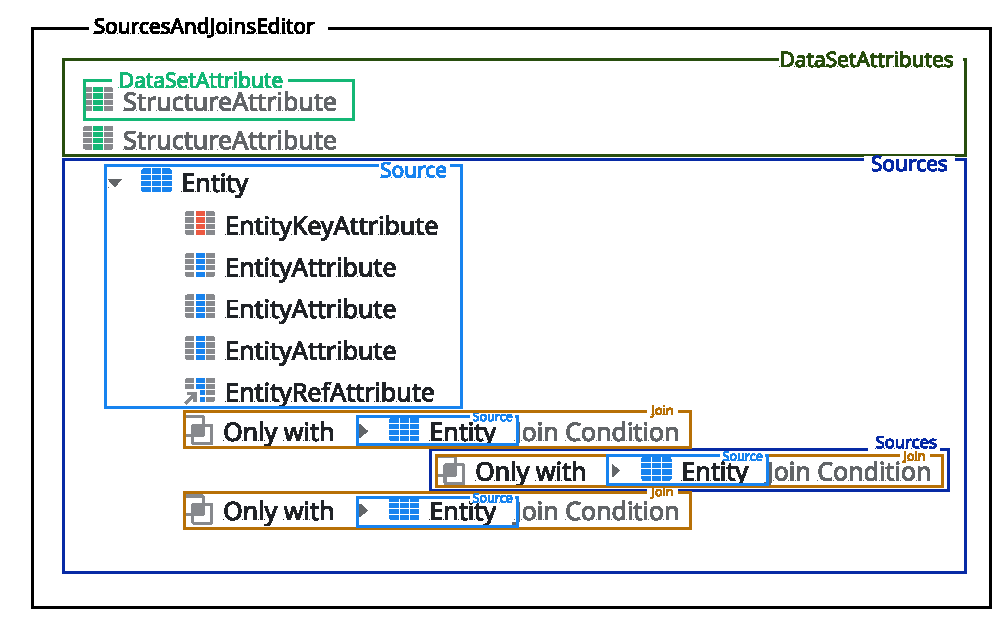
\includegraphics[height=3.0in]
  {sources-components-structure}
	\caption{Structure of the React components created to dispose the sources.}
	\label{fig:sourcesComponentsStructure}
\end{figure}

\subsection{Evaluation}
\label{subsec:service_studio_evaluation}

